% A LaTeX template for MSc Thesis submissions to 
% Politecnico di Milano (PoliMi) - School of Industrial and Information Engineering
%
% S. Bonetti, A. Gruttadauria, G. Mescolini, A. Zingaro
% e-mail: template-tesi-ingind@polimi.it
%
% Last Revision: October 2021
%
% Copyright 2021 Politecnico di Milano, Italy. NC-BY

\documentclass{Configuration_Files/PoliMi3i_thesis}
%------------------------------------------------------------------------------
%	REQUIRED PACKAGES AND  CONFIGURATIONS
%------------------------------------------------------------------------------

% CONFIGURATIONS
\usepackage{parskip} % For paragraph layout
\usepackage{setspace} % For using single or double spacing
\usepackage{emptypage} % To insert empty pages
\usepackage{multicol} % To write in multiple columns (executive summary)
\setlength\columnsep{15pt} % Column separation in executive summary
\setlength\parindent{0pt} % Indentation
\raggedbottom

% PACKAGES FOR TITLES
\usepackage{titlesec}
% \titlespacing{\section}{left spacing}{before spacing}{after spacing}
\titlespacing{\section}{0pt}{3.3ex}{2ex}
\titlespacing{\subsection}{0pt}{3.3ex}{1.65ex}
\titlespacing{\subsubsection}{0pt}{3.3ex}{1ex}
\usepackage{color}

% PACKAGES FOR LANGUAGE AND FONT
\usepackage[english]{babel} % The document is in English  
\usepackage[utf8]{inputenc} % UTF8 encoding
\usepackage[T1]{fontenc} % Font encoding
\usepackage[11pt]{moresize} % Big fonts

% PACKAGES FOR IMAGES
\usepackage{graphicx}
\usepackage{caption}
\usepackage{subcaption}
\usepackage{transparent} % Enables transparent images
\usepackage{eso-pic} % For the background picture on the title page
\usepackage{subfig} % Numbered and caption subfigures using \subfloat.
\usepackage{tikz} % A package for high-quality hand-made figures.
\usetikzlibrary{}
\graphicspath{{./Images/}} % Directory of the images
\usepackage{xcolor} % Coloured captions
\usepackage{amsthm,thmtools,xcolor} % Coloured "Theorem"
\usepackage{float}
\usepackage{pgfplots}
\pgfplotsset{compat=1.18}
% STANDARD MATH PACKAGES
\usepackage{amsmath}
\usepackage{amsthm}
\usepackage{amssymb}
\usepackage{amsfonts}
\usepackage{bm}
\usepackage[overload]{empheq} % For braced-style systems of equations.
\usepackage{fix-cm} % To override original LaTeX restrictions on sizes

% PACKAGES FOR TABLES
\usepackage{tabularx}
\usepackage{longtable} % Tables that can span several pages
\usepackage{colortbl}

\usepackage{listings}
\usepackage{multirow}

% PACKAGES FOR REFERENCES & BIBLIOGRAPHY
\usepackage[colorlinks=true,linkcolor=black,anchorcolor=black,citecolor=black,filecolor=black,menucolor=black,runcolor=black,urlcolor=black]{hyperref} % Adds clickable links at references
\usepackage{cleveref}

% OTHER PACKAGES
\usepackage{pdfpages} % To include a pdf file
\usepackage{afterpage}
\usepackage{lipsum} % DUMMY PACKAGE
\usepackage{booktabs}
\usepackage{enumitem}
\usepackage{fancyhdr} % For the headers
\usepackage{url}
\usepackage{matlab-prettifier}
\usepackage{minted}
\fancyhf{}

% Input of configuration file. Do not change config.tex file unless you really know what you are doing. 
% Define blue color typical of polimi
\definecolor{bluepoli}{cmyk}{0.4,0.1,0,0.4}

% Custom theorem environments
\declaretheoremstyle[
  headfont=\color{bluepoli}\normalfont\bfseries,
  bodyfont=\color{black}\normalfont\itshape,
]{colored}

% Set-up caption colors
\captionsetup[figure]{labelfont={color=bluepoli}} % Set colour of the captions
\captionsetup[table]{labelfont={color=bluepoli}} % Set colour of the captions

\theoremstyle{colored}
\newtheorem{theorem}{Theorem}[chapter]
\newtheorem{proposition}{Proposition}[chapter]

% Enhances the features of the standard "table" and "tabular" environments.
\newcommand\T{\rule{0pt}{2.6ex}}
\newcommand\B{\rule[-1.2ex]{0pt}{0pt}}

% Pseudo-code algorithm descriptions.
\newcounter{algsubstate}
\renewcommand{\thealgsubstate}{\alph{algsubstate}}
\newenvironment{algsubstates}
  {\setcounter{algsubstate}{0}%
   \renewcommand{\STATE}{%
     \stepcounter{algsubstate}%
     \Statex {\small\thealgsubstate:}\space}}
  {}

% New font size
\newcommand\numfontsize{\@setfontsize\Huge{200}{60}}

% Title format: chapter
\titleformat{\chapter}[hang]{
\fontsize{50}{20}\selectfont\bfseries\filright}{\textcolor{bluepoli} \thechapter\hsp\hspace{2mm}\textcolor{bluepoli}{|   }\hsp}{0pt}{\huge\bfseries \textcolor{bluepoli}
}

% Title format: section
\titleformat{\section}
{\color{bluepoli}\normalfont\Large\bfseries}
{\color{bluepoli}\thesection.}{1em}{}

% Title format: subsection
\titleformat{\subsection}
{\color{bluepoli}\normalfont\large\bfseries}
{\color{bluepoli}\thesubsection.}{1em}{}

% Title format: subsubsection
\titleformat{\subsubsection}
{\color{bluepoli}\normalfont\large\bfseries}
{\color{bluepoli}\thesubsubsection.}{1em}{}

% Shortening for setting no horizontal-spacing
\newcommand{\hsp}{\hspace{0pt}}

\makeatletter
% Renewcommand: cleardoublepage including the background pic
\renewcommand*\cleardoublepage{%
  \clearpage\if@twoside\ifodd\c@page\else
  \null
  \AddToShipoutPicture*{\BackgroundPic}
  \thispagestyle{empty}%
  \newpage
  \if@twocolumn\hbox{}\newpage\fi\fi\fi}
\makeatother

%----------------------------------------------------------------------------
%	NEW COMMANDS DEFINED
%----------------------------------------------------------------------------

% EXAMPLES OF NEW COMMANDS
\newcommand{\bea}{\begin{eqnarray}} % Shortcut for equation arrays
\newcommand{\eea}{\end{eqnarray}}
\newcommand{\e}[1]{\times 10^{#1}}  % Powers of 10 notation

%----------------------------------------------------------------------------
%	ADD YOUR PACKAGES (be careful of package interaction)
%----------------------------------------------------------------------------

%----------------------------------------------------------------------------
%	ADD YOUR DEFINITIONS AND COMMANDS (be careful of existing commands)
%----------------------------------------------------------------------------

%----------------------------------------------------------------------------
%	BEGIN OF YOUR DOCUMENT
%----------------------------------------------------------------------------

\usepackage[backend=biber]{biblatex}
\usepackage{csquotes}
\usepackage{hyperref} % For clickable links
\addbibresource{references.bib} % Link the bibliography file

\begin{document}

\fancypagestyle{plain}{%
\fancyhf{} % Clear all header and footer fields
\fancyhead[RO,RE]{\thepage} %RO=right odd, RE=right even
\renewcommand{\headrulewidth}{0pt}
\renewcommand{\footrulewidth}{0pt}}

%----------------------------------------------------------------------------
%	TITLE PAGE
%----------------------------------------------------------------------------

\pagestyle{empty} % No page numbers
\frontmatter % Use roman page numbering style (i, ii, iii, iv...) for the preamble pages

\puttitle{
	title = Homework Report, % Title of the thesis
	name = Salvi Niccolò, % First author
    ID = 10773726,  % Student ID number (numero di matricola)
    academicyear = 2024-25 % Academic Year
}

%----------------------------------------------------------------------------
%	LIST OF CONTENTS/FIGURES/TABLES/SYMBOLS
%----------------------------------------------------------------------------

% TABLE OF CONTENTS
\thispagestyle{empty}
\tableofcontents % Table of contents 
\thispagestyle{empty}
\cleardoublepage

\addtocontents{toc}{\vspace{2em}} % Add a gap in the Contents, for aesthetics
\mainmatter % Begin numeric (1,2,3...) page numbering

% --------------------------------------------------------------------------
% NUMBERED CHAPTERS % Regular chapters following
% --------------------------------------------------------------------------
\chapter{Image Processing}
The objective is to find straight lines, image of the circumference $C$ and the image of the unknown planar curve $S$ in the provided image.

\begin{figure}[H]
    \centering
    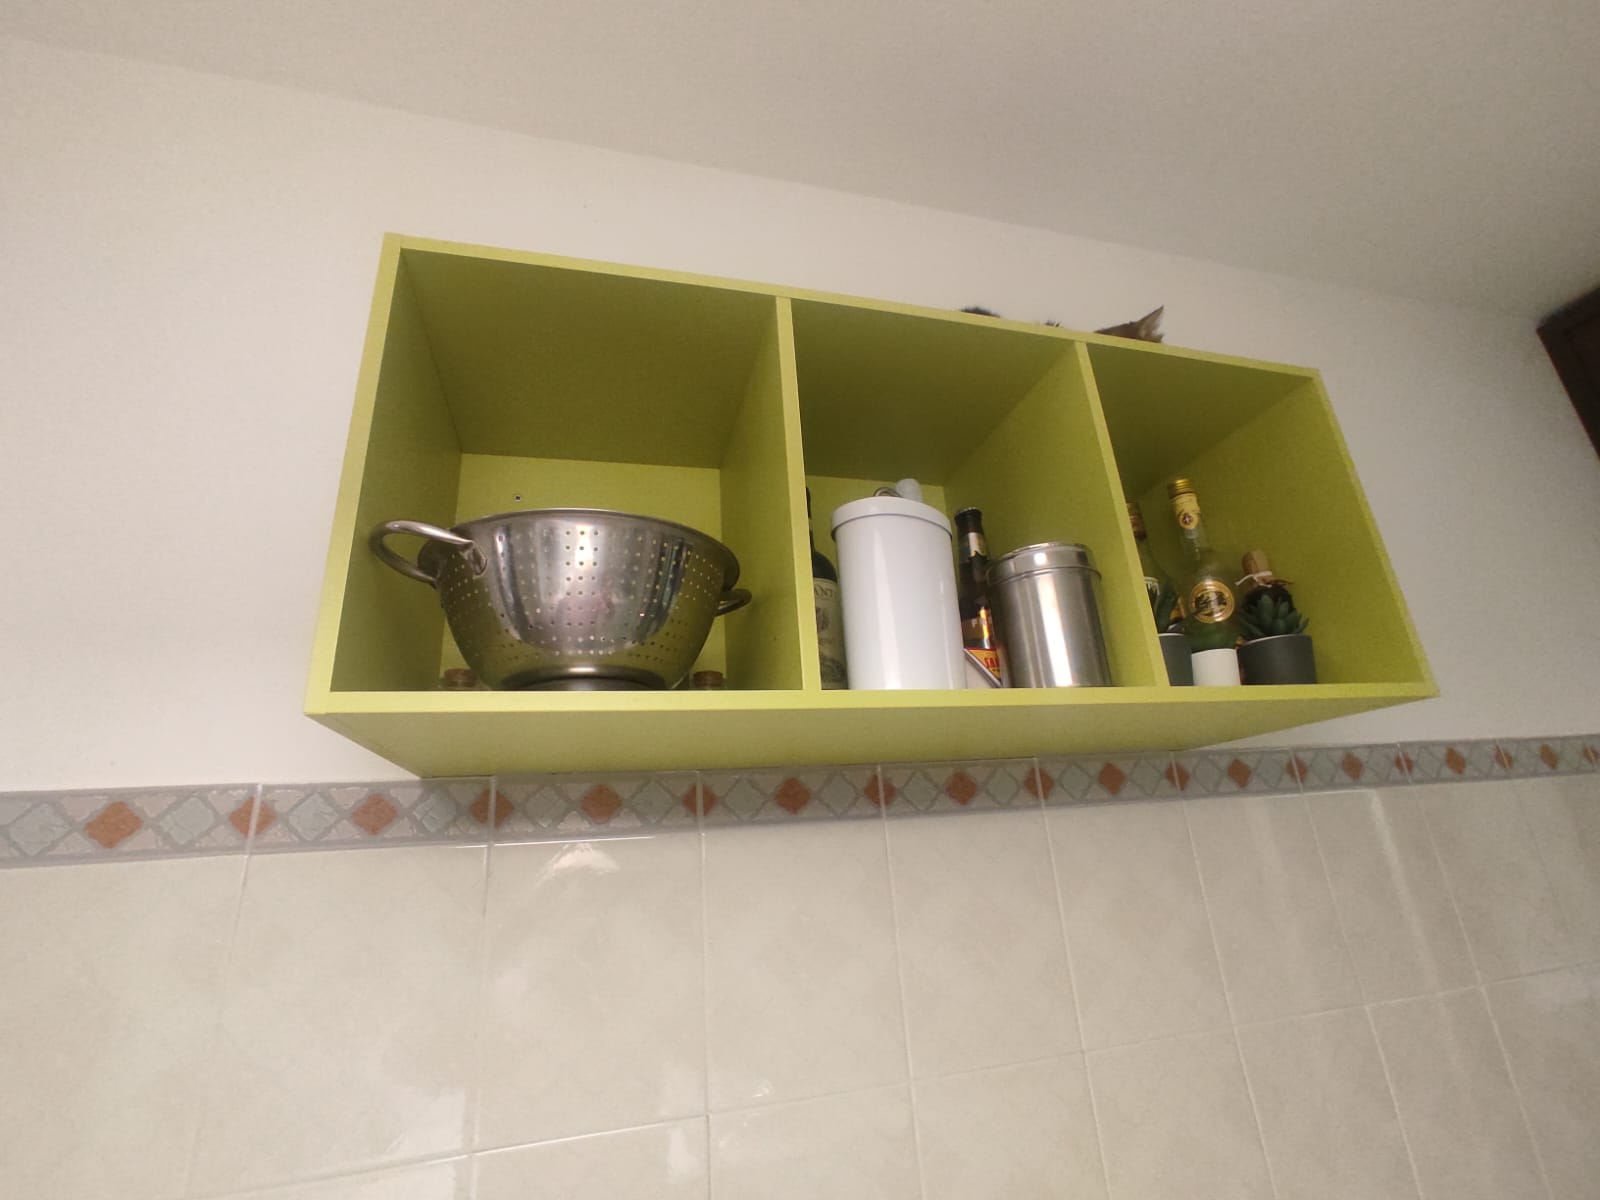
\includegraphics[width=0.75\linewidth]{img/Look-outCat.jpg}
    \caption{Original image}
    \label{fig:originalImage}
\end{figure}

\section{F1: Straight Line Detection}
The \textbf{Canny} method can be used to detect edges in the image. The algorithm works by first applying a smoothing Gaussian filter to the image (to remove noise), then computing the gradient of the image, applying nonmax suppression and tracking edges via hysteresis thresholding.
Matlab already includes (in the Image Processing Toolbox) an implementation for this method in the edge function.
First, we need to convert the image to grayscale. This way, the resulting image matrix will contain doubles in the [0,1] interval, representing the "intensity" of each pixel.

\begin{minted}{matlab}
img = im2double(imread('look-outCat.jpg'));
imgGrayscale = rgb2gray(img);
\end{minted}

Then we can simply use the edge function to apply the Canny method. A threshold can be specified to adjust the output image; in our case a value of [0.05, 0.2] seems to yield the best results.
\begin{minted}{matlab}
BW = edge(Igray, 'canny', [0.05, 0.2]);
\end{minted}

The result is pretty good, since we are able to identify some of the requested lines.
\begin{figure}[H]
    \centering
    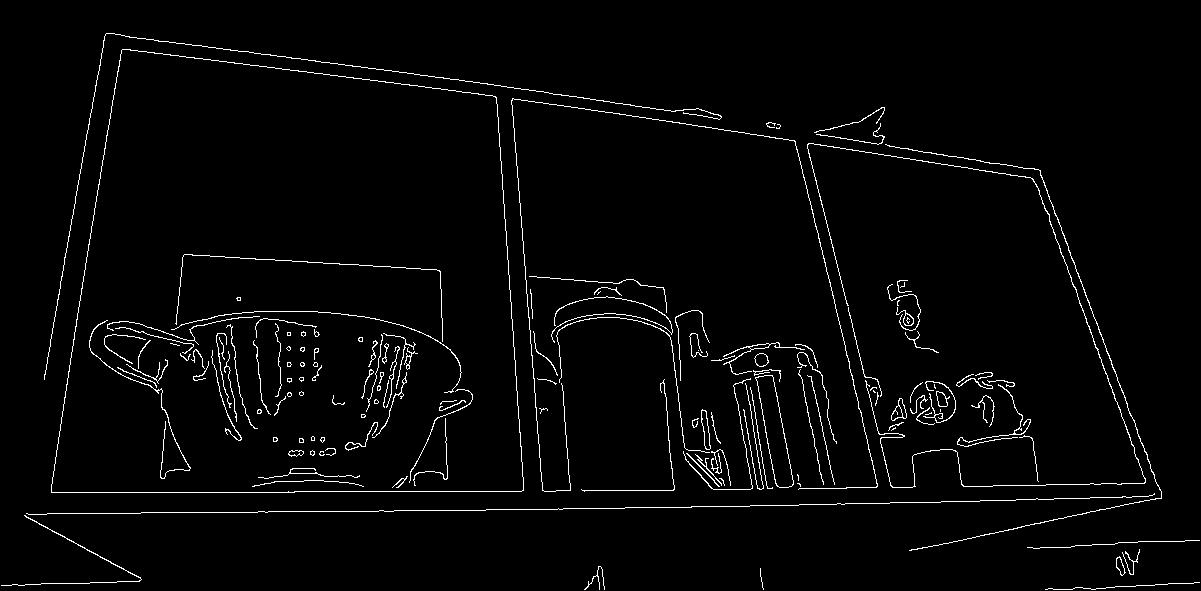
\includegraphics[width=0.75\linewidth]{img/imageProcessing/BW.jpg}
    \caption{Canny}
    \label{fig:canny}
\end{figure}

We can use the results of the previous step to detect straight lines in the image. This can be done using the \textbf{Hough transform}. A Hough transform of a datum (in this case a point on a detected edge) is a set of models compatible with the datum in the \emph{model space}.
For a point in the cartesian plane, the HT will be a sinusoid; collinear points will map to (almost) concurrent HTs.

The Hough transform is also included in Matlab:
\begin{minted}{matlab}
[H, T, R] = hough(edges);
\end{minted}
where \verb|T| is $\theta$, \verb|R| is $\rho$ and \verb|H| is a matrix whose rows and columns correspond to $\rho$ and $\theta$ values respectively.

We can then use the \verb|houghpeaks| function to detect peaks, and pass the results to \verb|houghlines| to extract lines.
\begin{minted}{matlab}
P = houghpeaks(H, 100, 'threshold', 0.3*max(H(:)));
hlines = houghlines(edges, T, R, P, 'FillGap', 4, 'MinLength', 14);
\end{minted}

These functions include various configuration options, namely:
\begin{itemize}
	\item \verb|numpeaks| is the number of peaks to detect (set to 20 here)
	\item \verb|threshold| is the minimum value to be considered a peak. By default it is set to half the maximum value in the \verb|H| matrix. For our image, we can get better results by lowering it to 30\% of the max value.
	\item \verb|FillGap| is, quoting the Matlab documentation, \emph{the distance between two line segments associated with the same Hough transform bin}. In practice, this value controls the max distance between two detected segments for them to be merged into one segment.
	\item \verb|MinLength| controls the minimum length for a segment. Setting this to a higher value allows to remove some bad segments in noisy areas of the image (e.g. the hedge).
\end{itemize}

The parameters detailed above can be adjusted based on whether we want a cleaner output or more/longer lines in the output.

\begin{figure}[H]
    \centering
    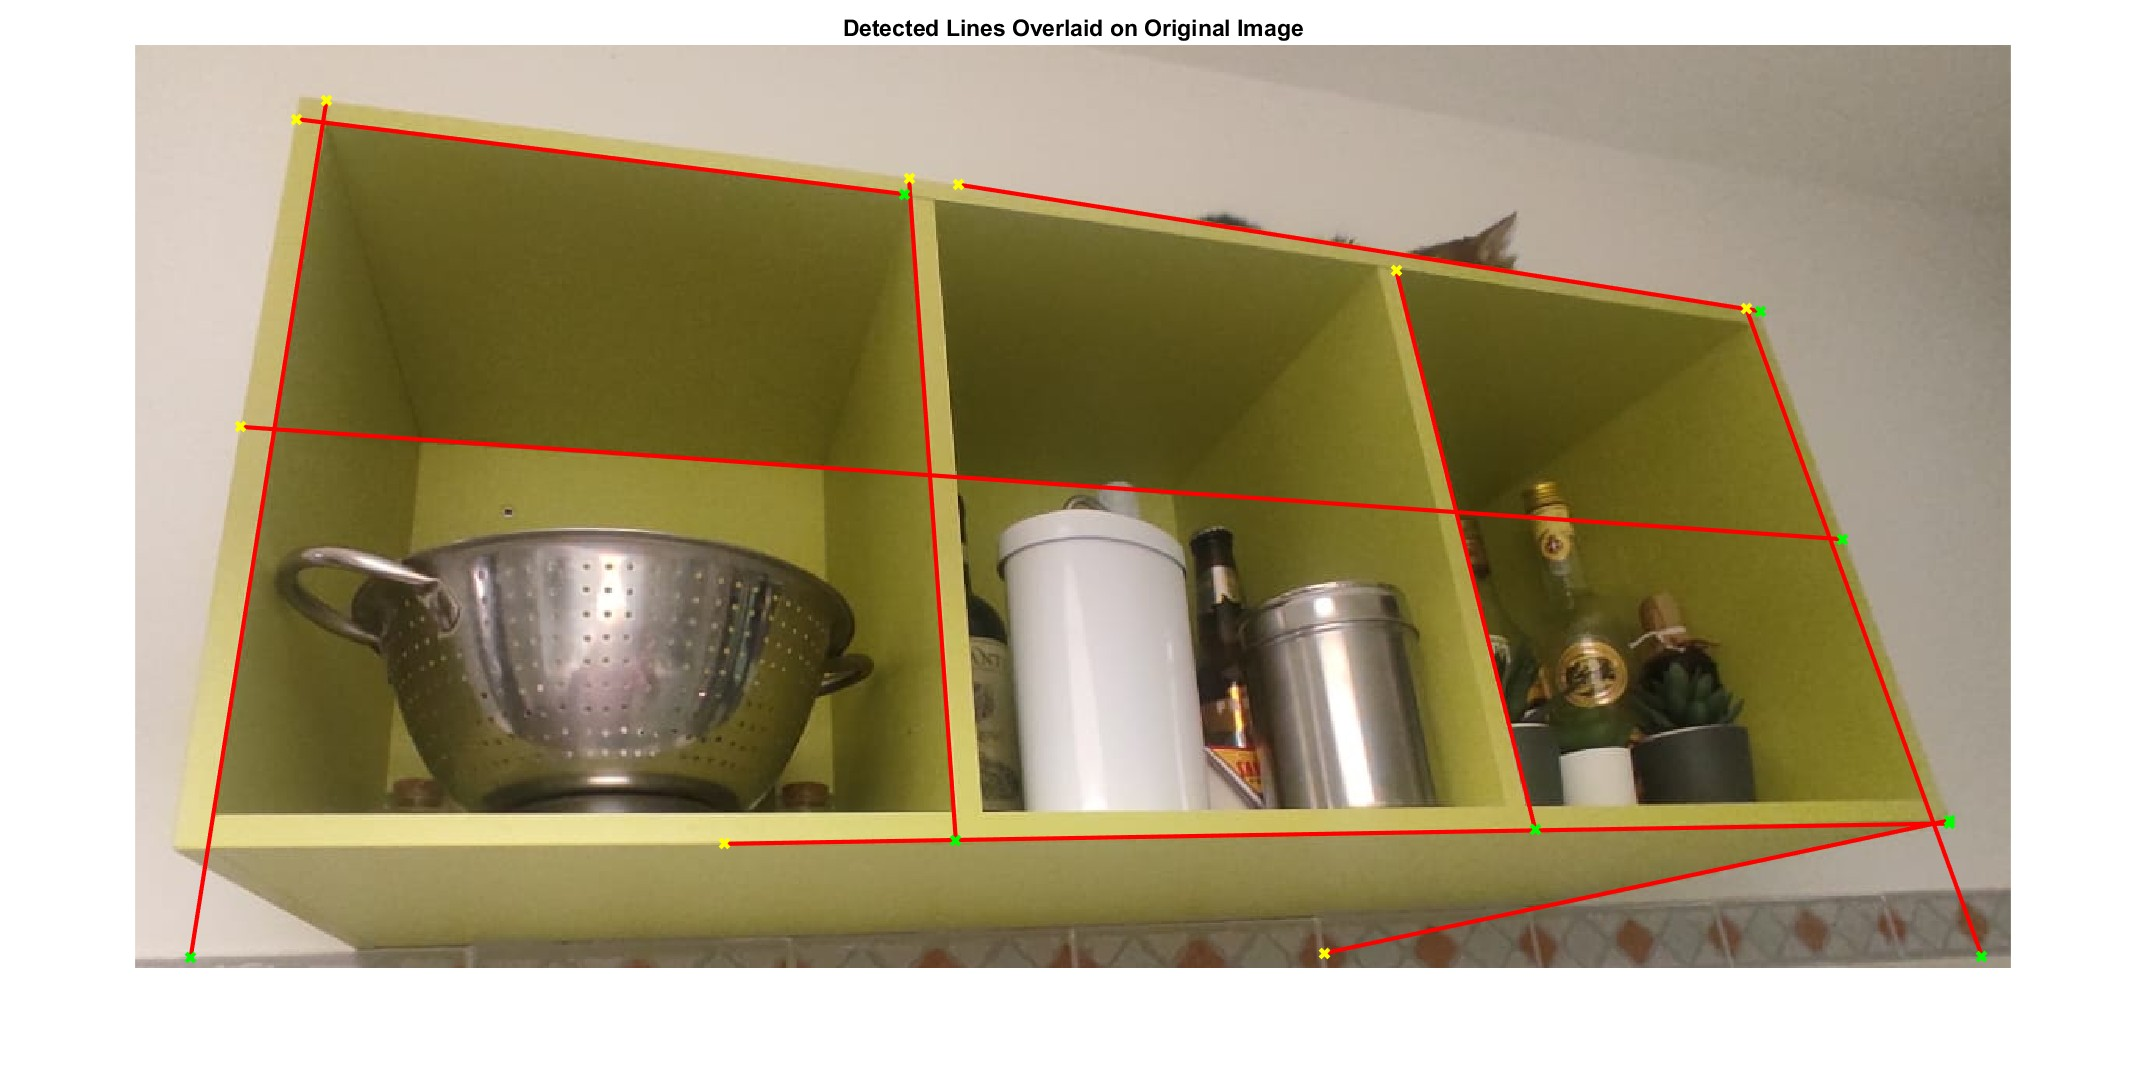
\includegraphics[width=0.75\textwidth]{img/imageProcessing/DetectedLines.jpg}
    \caption{Straight lines detected with the Hough Transform}
    \label{fig:detectStraightLines}
\end{figure}

To conclude, we were able to find precisely \verb|h| lines and some of the \verb|l| lines. The worst result is for \verb|m| lines, but increasing the contrast between dark and light areas, we could find any additional and useful edges.

\section[F2: Image of \textit{C}]{F2: Image of $C$}\label{sec:detectedC}
The goal of this task was to find the image of the circumference \verb|C| from the provided image. The task involved identifying the conic equation of the circumference based on a set of manually selected points and subsequently visualizing the computed conic on the original image.

To achieve this, the following steps were taken:

\paragraph{Point Selection:} Instead of using an interactive tool like 'getpts`, the points on the circumference were pre-defined for consistency and precision:
\begin{minted}{matlab}
   x = [417.9118, 437.6296, 456.3276, 585.1732, 721.4981, 724.8977]
   y = [566.9941, 581.6125, 526.1986, 510.9003, 543.1967, 592.1513]
\end{minted}
These points were selected manually based on the visible circumference in the image.

\paragraph{Fitting the Conic Equation:} The general conic equation is expressed as:
$$
ax^2 + bxy + cy^2 + dx + ey + f = 0
$$
To determine the coefficients $(a, b, c, d, e, f)$, a design matrix $A$ was constructed from the selected points:
$$
A = \begin{bmatrix} 
x_1^2 & x_1y_1 & y_1^2 & x_1 & y_1 & 1 \\
x_2^2 & x_2y_2 & y_2^2 & x_2 & y_2 & 1 \\
\vdots & \vdots & \vdots & \vdots & \vdots & \vdots
\end{bmatrix}
$$
The coefficients were estimated by solving $A \cdot c = 0$ using Singular Value Decomposition (SVD). The last column of the $V$ matrix from the SVD provided the solution.

\paragraph{Conic Matrix Representation:} The coefficients were used to construct the conic matrix $C$:
$$
C = \begin{bmatrix} 
a & \frac{b}{2} & \frac{d}{2} \\ 
\frac{b}{2} & c & \frac{e}{2} \\ 
\frac{d}{2} & \frac{e}{2} & f
\end{bmatrix}
$$
The matrix was normalized by dividing all elements by $C(3, 3)$.

\begin{figure}[H]
    \centering
    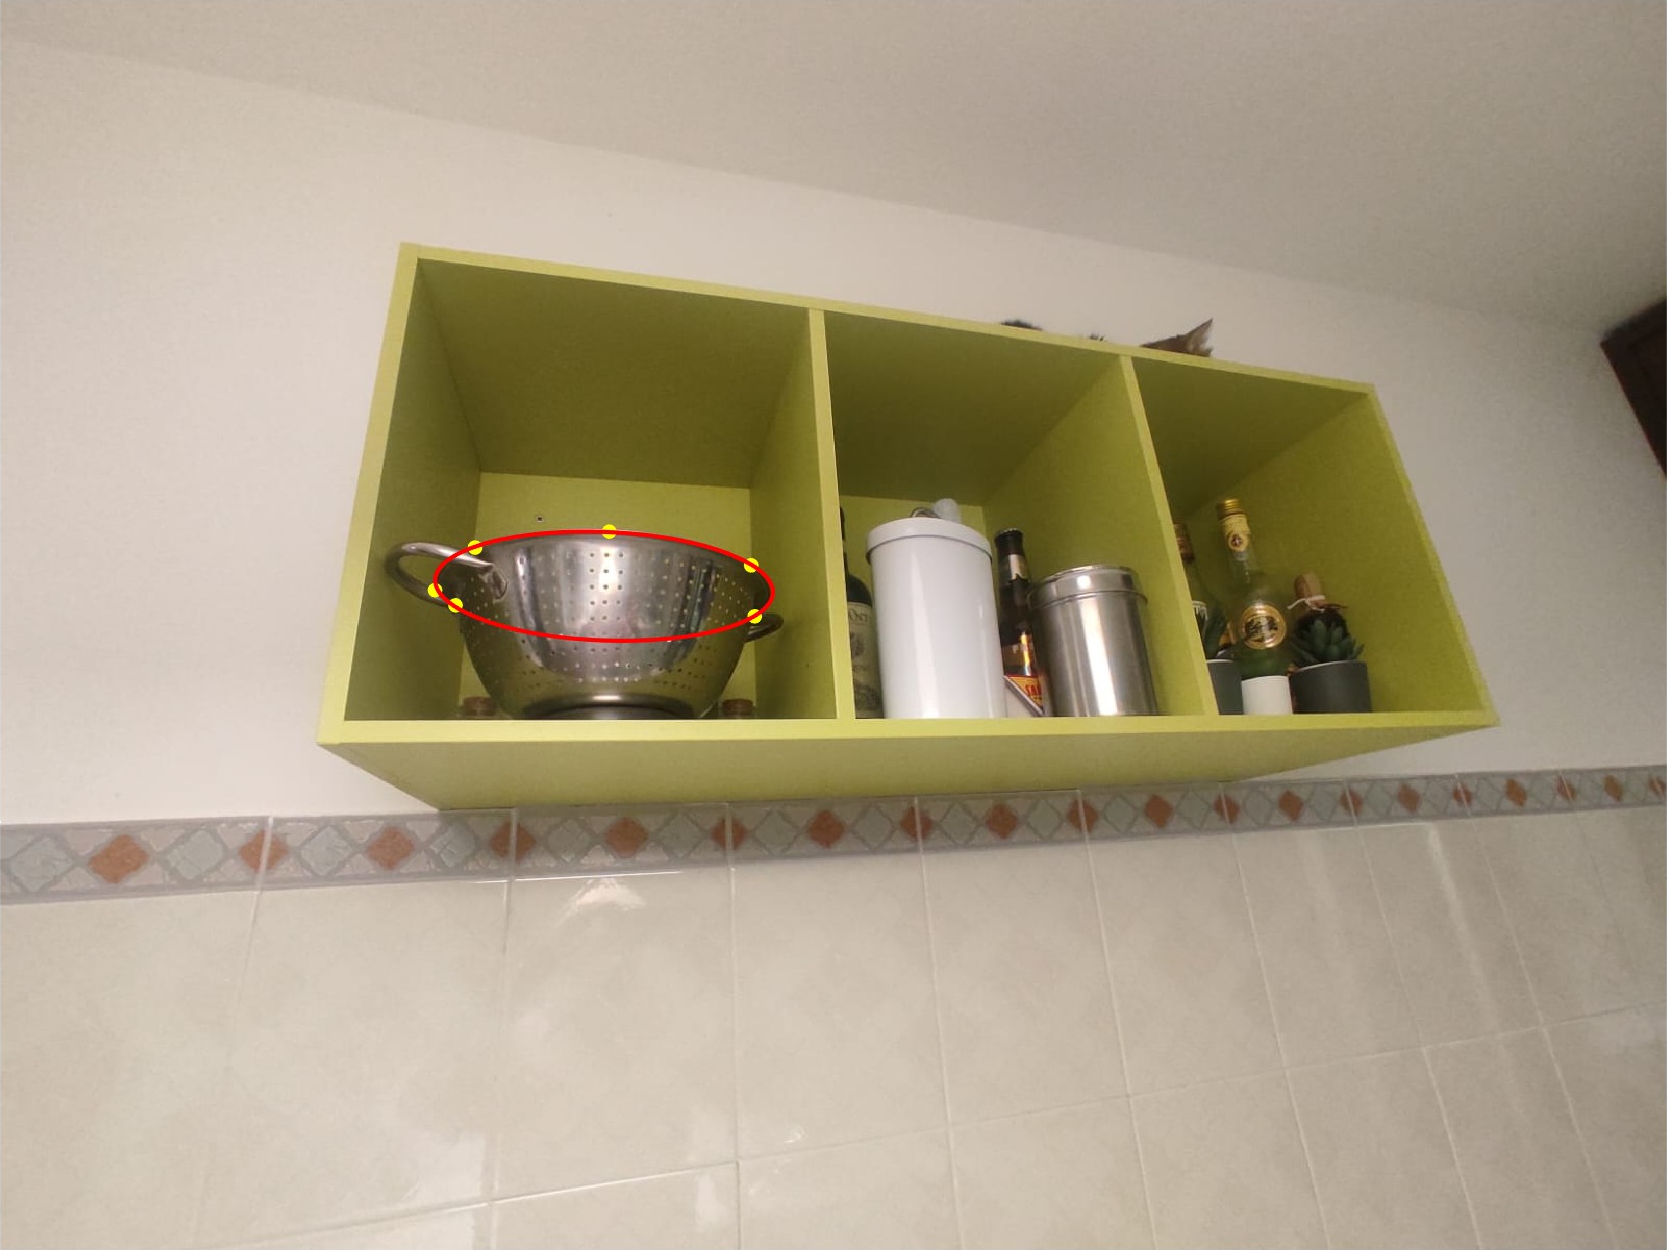
\includegraphics[width=0.75\textwidth]{img/imageProcessing/detected_conic.jpg}
    \caption{Detected conic $C$}
    \label{fig:detectedC}
\end{figure}

\section[F3: Image of \textit{S}]{F3: Image of $S$}
The goal of this task was to identify and visualize the image of a unknown curve $S$ in the provided image. This involved detecting edge points, robustly fitting an ellipse to these points using the \textbf{RANSAC} (Random Sample Consensus) algorithm, and plotting the detected curve over the original image. To focus on the elliptical curve $S$, the edge points were restricted to a predefined region of interest (ROI). This eliminated irrelevant edges outside the region containing the curve.

RANSAC was used to robustly fit an ellipse to the detected edge points in the ROI. The algorithm iteratively selects random subsets of points, fits a candidate ellipse, and identifies inliers based on their proximity to the candidate.
The best-fitting ellipse was refined by re-fitting to all inliers identified in the final RANSAC iteration.

The fitted ellipse parameters (center, axes, and orientation) were used to plot the curve $S$ as a partial ellipse. The visualization highlighted the curve on the original image, restricted to a specific segment based on its geometric properties.

The RANSAC algorithm successfully identified the elliptical curve $S$, even in the presence of noise and irrelevant edge points. The fitted ellipse was visualized as a partial curve restricted to the ROI, with endpoints refined based on geometric criteria.

I thought also to another way to solve the task, using a similar approach to what we have been used to complete the previous task, using the function \texttt{spline()} after selected manually some points on the curve.

\begin{figure}[H]
    \centering
    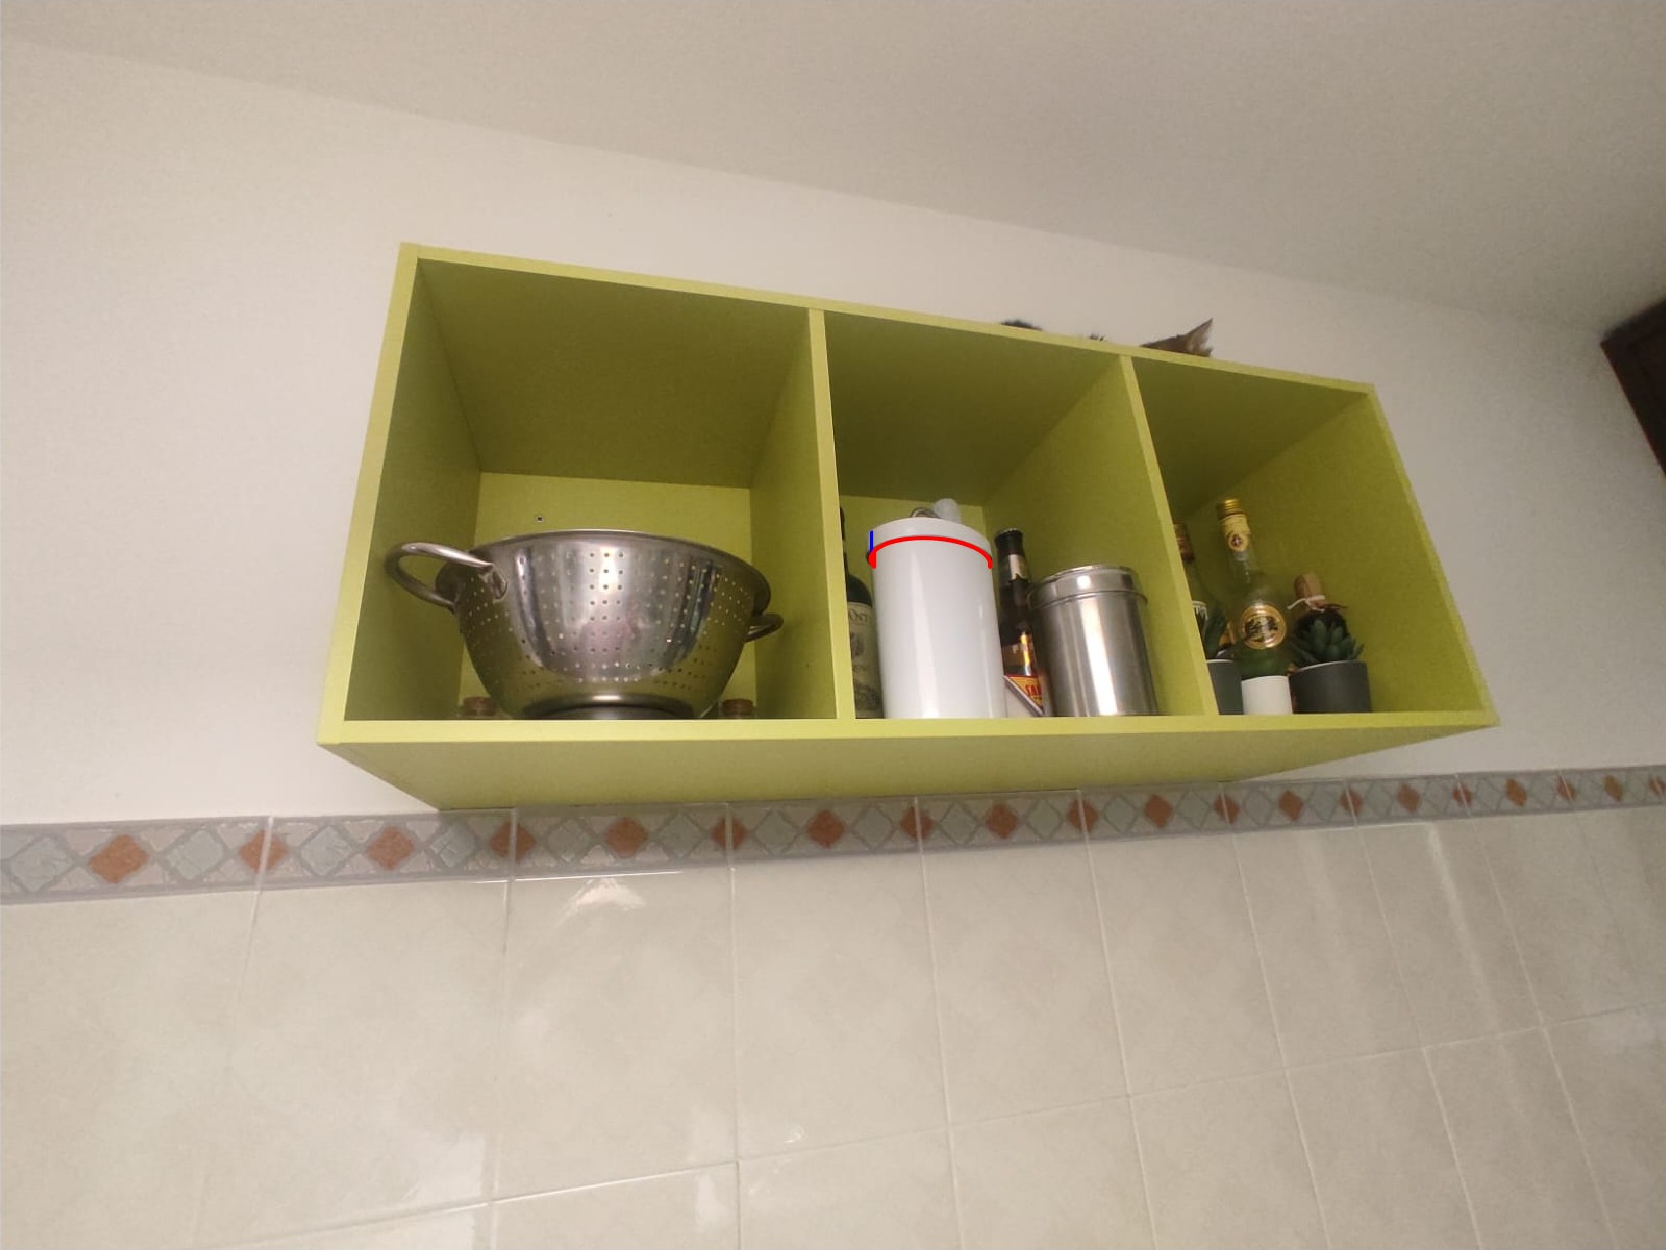
\includegraphics[width=0.75\textwidth]{img/imageProcessing/detected_s.jpg}
    \caption{Detected unknown curve $S$}
    \label{fig:detectS}
\end{figure}

\chapter{Geometry}
\section{G1 - Estimation of vanishing line of the horizontal plane}\label{infLine}
In projective geometry, a vanishing point is the image of a set of parallel lines in \verb|3D| space after projecting onto the \verb|2D| image plane. Although truly parallel lines in the scene never meet in Euclidean space, their perspective projection often appears to converge at a single point in the image.

Due to measurement noise and inaccuracies, different pairs of parallel lines will not intersect at a single precise point. Thus, a common strategy is to seek the point that minimizes the sum of squared distances between the measured image lines and a single convergent point, leading to a maximum likelihood estimate under Gaussian noise assumptions.

Although the initial request was to automatically extract straight lines, I opted to manually select all the required lines to achieve a more accurate and precise outcome.

\subsection[Vanishing Point of \textit{l} Lines]{Vanishing Point of $l_i$ Lines} \label{sec:vanPoint_l}
In the following section there will be presented two different approaches to estimate the vanishing point of $l_i$ lines. 

\subsubsection{Centroid-based Approach}
The centroid-based approach is a simple and computationally efficient method for estimating the vanishing point in an image. It involves computing the intersections of all pairs of image lines and taking the centroid (mean position) of these intersection points as the estimated vanishing point.

Despite its simplicity, the centroid method lacks robustness to noise and outliers, as all intersections are treated equally, including those from erroneously detected lines. As such, it is best suited for cases where line measurements are precise and free from significant outliers. For higher accuracy, more advanced methods, such as optimization-based techniques, are preferred.

\subsubsection{Levenberg-Marquardt Algorithm}
The Levenberg-Marquardt (LM) algorithm is a popular technique for solving non-linear least squares problems. It combines the best features of two optimization methods: the Gauss-Newton method and gradient descent.

\begin{itemize}
    \item \textbf{Gauss-Newton:} Efficient for problems that are well approximated by a quadratic near the solution, using the Jacobian and approximate second-order information.
    \item \textbf{Gradient Descent:} Robust for initial steps, but can be slow to converge.
\end{itemize}

LM smoothly transitions between these two approaches. When the solution is far from the optimum, LM behaves more like gradient descent, ensuring stability. As it gets closer to the optimum, it behaves more like Gauss-Newton, ensuring fast convergence. This makes LM a robust and efficient choice for a variety of parameter estimation problems, including camera calibration, structure-from-motion, and vanishing point estimation.

\subsubsection{Comparison and results}
In our scenario, the image data and detected lines exhibit relatively low levels of noise, as the parallel structures in the scene are well-defined and the line detections are accurate. As a result, the intersections of the lines cluster closely around the true vanishing point, minimizing the scatter typically caused by noise.

Given these favourable conditions, the centroid-based approach provides a computationally efficient and sufficiently accurate method for estimating the vanishing point. As demonstrated in the accompanying figure, the centroid of the pairwise line intersections aligns closely with the true vanishing point, delivering reliable results without requiring more complex optimization methods like the Levenberg-Marquardt algorithm.

While the LM algorithm offers improved robustness and precision in highly noisy or challenging datasets, in this case, its additional computational overhead is unnecessary. The simplicity and effectiveness of the centroid-based method make it the preferred choice for this specific scenario.

The vanishing points of $l$ lines we found:
$$
V_{l_{centroid}} = [3392.3, \, 666.4, \, 1]^T \qquad V_{l_{LM}} = [3416.8, \, 674.4, \, 1]^T
$$

The computed values are very similar; therefore, for the subsequent steps, we will use the $V_l$ value obtained through the centroid-based approach.

$$V_l = [3392.3, \, 666.4, \, 1]^T$$

\subsection[Vanishing Point of \textit{m} Lines]{Vanishing Point of $m_j$ Lines}
Similarly to the previous section and based on the result's comparison between LM approach and centroid-based one, I estimate the vanishing point of $m_j$ lines using the centroid based approach:

$$
V_m = [581.4, \, 883.8, \, 1]^T
$$

\subsection{Estimation of the line at infinity}
The task was to construct and visualize the \textbf{line at infinity} $l'_\infty$ in the image plane, given the coordinates of two vanishing points. 

The line passing through the two vanishing points is computed using \textbf{cross product}
$$l_\infty = V_l \times V_m$$
where $V_l$ and $V_m$ are represented in homogeneous coordinates.

The result vector $l'_\infty = [a, \, b, \, c]^T$ represents the line at infinity in homogeneous coordinates, where:
$$ax + by + c = 0$$

The obtained result is:
$$l'_\infty = [-0.0001, \, -0.0011, \, 1]^T $$
\begin{figure}[H]
    \centering
    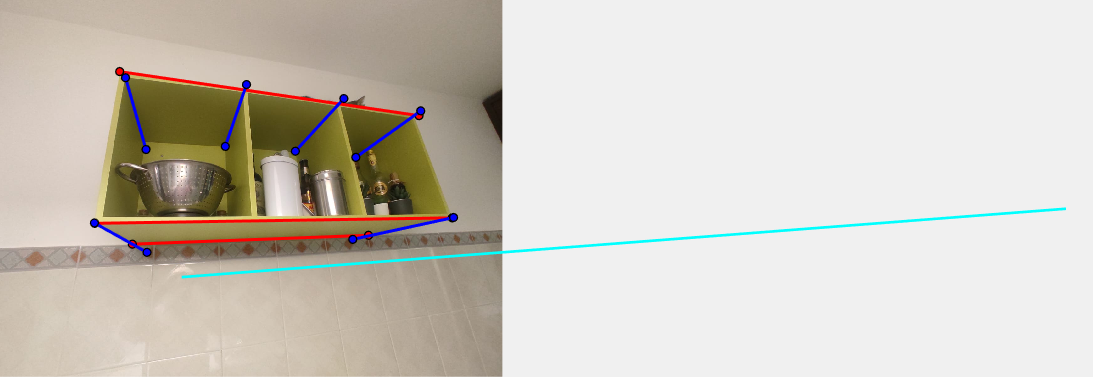
\includegraphics[width=0.95\linewidth]{img/G1/line_at_infinity.jpg}
    \caption{Line at Infinity}
    \label{fig:lineAtInfinity}
\end{figure}
\section{G2: 2D reconstruction of the horizontal plane}
In the following section we are going to explore several ways to obtain a metric rectification of the original image.

In order to establish which are the possible and navigable ways to compute the metric rectification of our original image, we list the detected object in our image that could help us to achieve our objective:
\begin{itemize}
    \item 3 independent families of orthogonal lines: $l_i$, $m_j$ and $h_k$ lines; we know they are orthogonal each other since they represents the three axis in the original \verb|3D| scene
    \item the horizontal circumference $C$
    \item the unknown planar curve $S$
\end{itemize}

\bigbreak

Based on the available objects, we can compute the desired metric rectification using two different methods:
\begin{itemize}
    \item metric-stratified method
    \item metric rectification using one circle
\end{itemize}

We can't use the method involving 5 pairs of orthogonal lines, because we haven't the necessary pairs of independent orthogonal lines; we have only 3, as reported previously.

\subsection{Metric stratified method}
The metric stratified method consists of first performing an affine rectification and then finding $C_{\infty}^{*'}$ through two more constraints.
\subsubsection{Affine rectification}
By selecting two independent pairs of parallel lines in the original image scene, we can estimate their intersection using the cross product. This allows us to determine the image of the line at infinity that connects the resulting vanishing points.

The goal of affine rectification is to map the image of the line at infinity to its canonical position, thereby preserving and restoring the parallelism of lines. This is a direct result of aligning the line at infinity with its original position.

Since our objective is to compute a 2D reconstruction of the horizontal plane, the lines to be selected are $l_i$ and $m_j$, for which we have already computed $l_{\infty}'$ in the previous section (\ref{infLine}).

The computed affine-homography matrix is the following:
\[
    H_{aff}
    =
    \begin{bmatrix}
        1.0000 & 0 & 0 \\
        0 & 1.0000 & 0 \\
        -0.0001 & -0.0011 & 1.0000
    \end{bmatrix}
\]

The affine rectified image is shown below:
\begin{figure}[H]
    \centering
    \includegraphics[width=0.75\linewidth]{img/affineRectifiedImage.jpg}
    \caption{Affine rectified image}
    \label{fig:affineRectification}
\end{figure}

\subsubsection{Metric rectification using imaged right angles}
After obtaining the affine rectified image, two additional constraints are necessary to address the two degrees of freedom associated with the circular points. These constraints allow the computation of a metric rectification, which restores the metric properties of the world plane.

One approach to derive these constraints is by identifying two imaged right angles on the world plane. In the affine rectified image, let $l'$ and $m'$ represent an orthogonal line pair $l$ and $m$ on the world plane. The orthogonality condition can then be leveraged, where the cosine of the angle between two lines is given by:

\begin{equation}
    \cos\theta = \frac{l^{'T} C_\infty^{*'} m^{'}}{\sqrt{(l^{'T} C_\infty^{*'} l^{'}) (m^{'T} C_\infty^{*'} m^{'})}} \label{eq:1}
\end{equation}

Since $l$ and $m$ are orthogonal, $\cos \theta = 0$, which simplifies to:

\[
    l^{'T} C_\infty^{*'} m^{'} = 0
\]

By substituting the definition of $C_\infty^{*'}$, the constraint becomes:

\[
    (l'_1 \quad l'_2 \quad l'_3)
    \begin{bmatrix}
        KK^T & 0 \\
        0^T & 0
    \end{bmatrix}
    \begin{pmatrix}
        m'_1 \\
        m'_2 \\
        m'_3
    \end{pmatrix}
    = 0
\]

This equation establishes the necessary relationship to constrain the circular points and achieve metric rectification.

Despite selecting two independent pairs of orthogonal lines, as illustrated in the following image, we were unable to compute the rectified image due to likely numerical errors.


\begin{figure}[H]
    \centering
    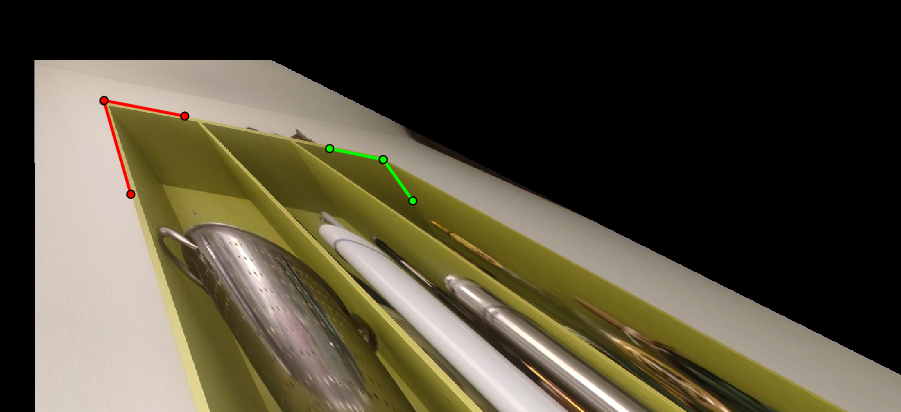
\includegraphics[width=0.75\linewidth]{img/G2/tryMetric.jpg}
    \caption{Two independent pairs of orthogonal lines}
    \label{fig:twoPairsOfOrthogonalLines}
\end{figure}

In conclusion, a different approach must be adopted to achieve the metric rectification of the provided image.

\subsection{Metric rectification using one circle}
Having detected the circumference $C$ in section (\ref{sec:detectedC}), we can use this information to compute the metric rectification.

The image of the circular points is determined by the intersection of the conic $C$ and the line at infinity $l_\infty'$. This intersection corresponds to the points on the conic that lie at infinity in the projective plane.

\paragraph{Conic equation} A general conic in homogeneous coordinates $[x, y, 1]^T$ is represented as:
$$C(x,y) = ax^2 + bxy + cy^2 + dx + ey + f = 0$$
Where $C$ if the conic matrix:
\[
    C
    =
    \begin{bmatrix}
        a & b/2 & d/2 \\
        b/2 & c & e/2 \\
        d/2 & e/2 & f
    \end{bmatrix}
    = 
     \begin{bmatrix}
        -3.20 \times 10^{-7} & \frac{2.12 \times 10^{-7}}{2} & \frac{2.53 \times 10^{-4}}{2} \\
        \frac{2.12 \times 10^{-7}}{2} & -3.06 \times 10^{-6} & \frac{3.32 \times 10^{-3}}{2} \\
        \frac{2.53 \times 10^{-4}}{2} & \frac{3.32 \times 10^{-3}}{2} & -1.00
    \end{bmatrix}
\]

\paragraph{Line at infinity} The line at infinity $l'_\infty$ in homogeneous coordinates is expressed as:
$$l'_\infty(x, y) = l_1x + l_2y + l_3 = 0$$

\paragraph{System of equations}
The intersection of the conic and the line at infinity is obtained by solving the following system of equations:
\begin{itemize}
    \item Conic equation:
    $$ax^2 + bxy + cy^2 + dx + ey + f = 0$$
    \item Line at infinity:
    $$l_1x + l_2y + l_3 = 0$$
\end{itemize}

\paragraph{Circular points in homogeneous coordinates} The resulting points in homogeneous coordinates are:
\[
    s_1 = \begin{bmatrix}
        x_1 \\
        y_1 \\
        1
    \end{bmatrix}, \quad
    s_2 = \begin{bmatrix}
        x_2 \\
        y_2 \\
        1
    \end{bmatrix}
\]
These points correspond to the \textbf{image of the circular points}.

The computed circular points are complex conjugates, as they lie on the real conic and at infinity. Their representation enables constructing the \textbf{dual conic of the circular points}:

$$C_\infty' = s_1s_2^T + s_2s_1^T$$

The final metric rectification matrix $H_{met}$ obtained is:
\[
    \label{metricRectMatrix}
    H_{met}
    =
    \begin{bmatrix}
        1.4243 & -6.9489 \times 10^{-1} & 0 \\
        -6.9489 \times 10^{-1} & 2.1380 & 0 \\
        -1.0000 \times 10^{-4} & -1.1000 \times 10^{-3} & 1
    \end{bmatrix}
\]

and the final metric rectified image is:
\begin{figure}[H]
    \centering
    \includegraphics[width=0.75\linewidth]{img/G2/metric_rectified_image.jpg}
    \caption{Metric rectified image using $C$}
    \label{fig:metricRectificationUsingOneCircle}
\end{figure}

\subsection[Estimation of \textit{m} Lines]{Estimation of $m$}\label{estimationDepth}
To compute the depth $m$ of the parallelepiped, we start by considering its known length $l = 1 \, m$. Using the lines \textit{l} and the hypotenuse of the triangle and the angle $\alpha$ between them (refer to the accompanying illustrations for clarity), we calculate $\cos\alpha$ using equation \ref{eq:1}.

From the metric rectified image, we observe that $l$ and $m$ are orthogonal, forming a right triangle. According to the properties of a right triangle, the depth $m$ can be expressed as:

$$ m = l \sin\alpha$$

Given $\cos\alpha$, we compute $\sin\alpha$ using the trigonometry identity:
$$\sin\alpha =  \sqrt{1-\cos^2\alpha}$$

Substituting the calculated values, we find:
$$m \approx \frac{1}{3} \, m$$

\begin{figure}[H]
    \centering
    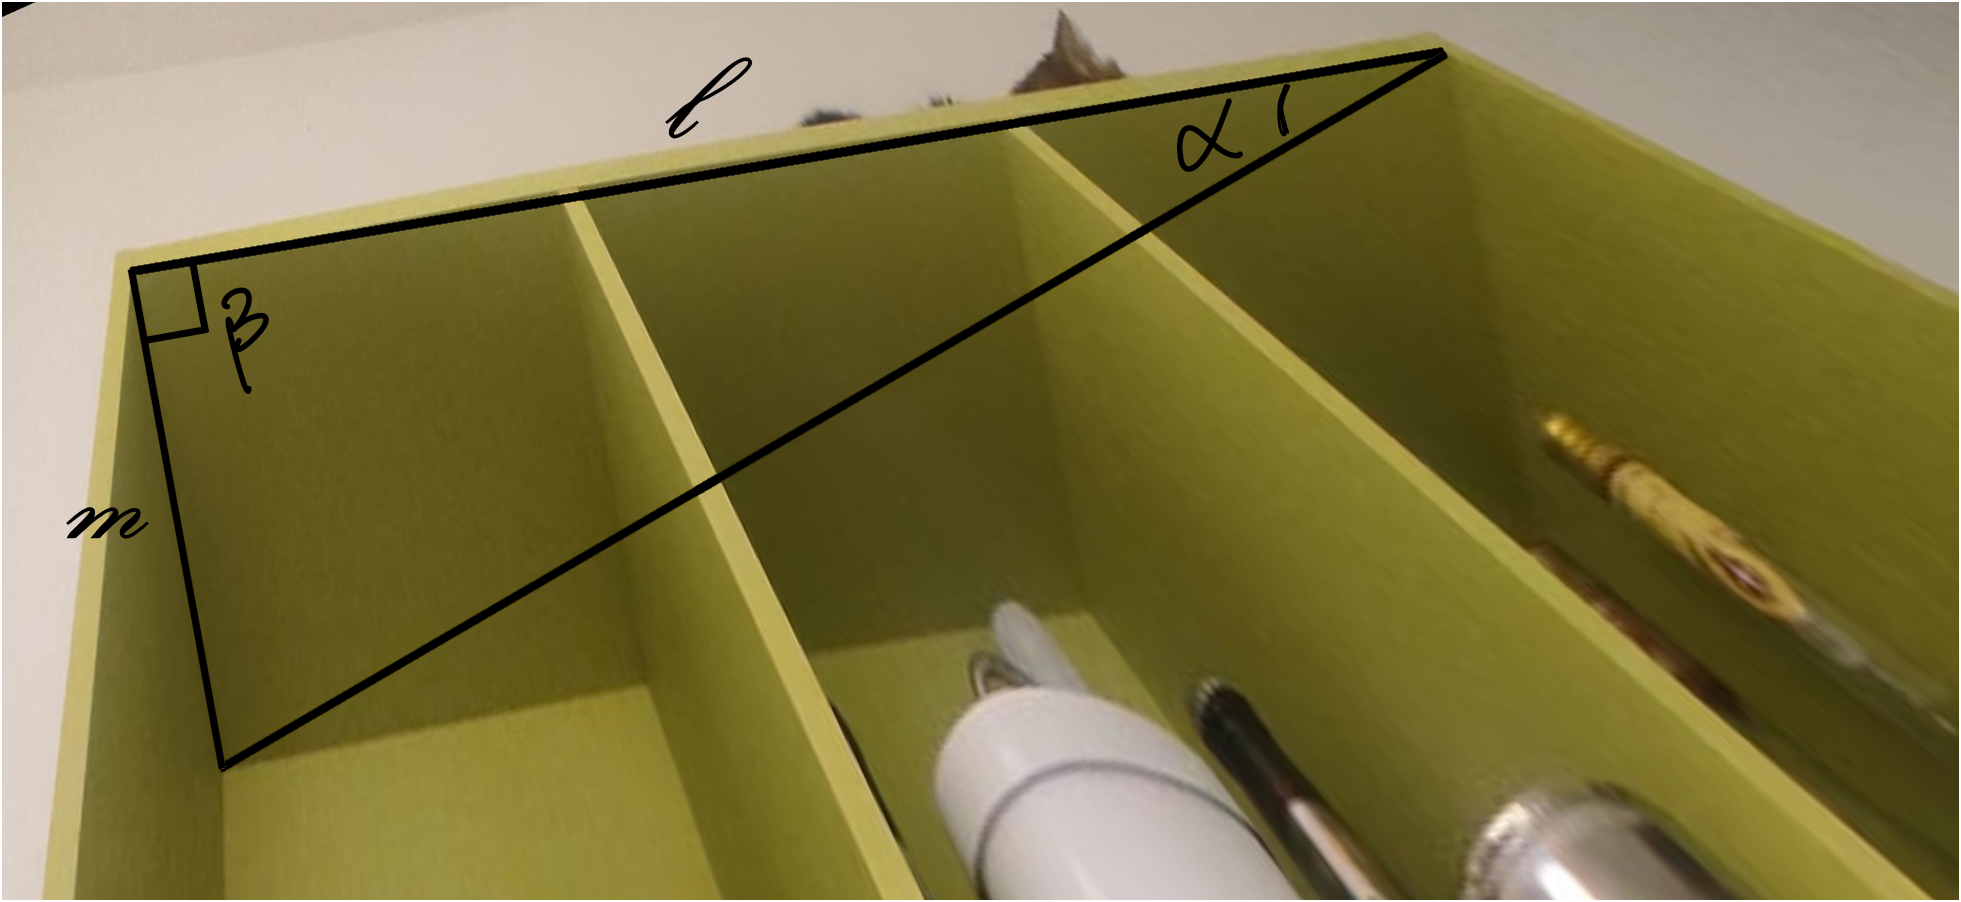
\includegraphics[width=0.7\linewidth]{img/triangleWithAngles.png}
    \caption{Triangle in metric rectified image}
    \label{fig:triangleWithAngles}
\end{figure}

\subsubsection{Double check of the result}
To double check the obtained result, we start doing an hypothesis: the parallelepiped is divide into three parts of equals length.
\paragraph{Compute cross ratio}
To prove it, we need to compute the cross ratio (\textit{CR}) of every divisor, between points $A$, $B$, $C$, $D$ shown in the following image.

\begin{figure}[H]
    \centering
    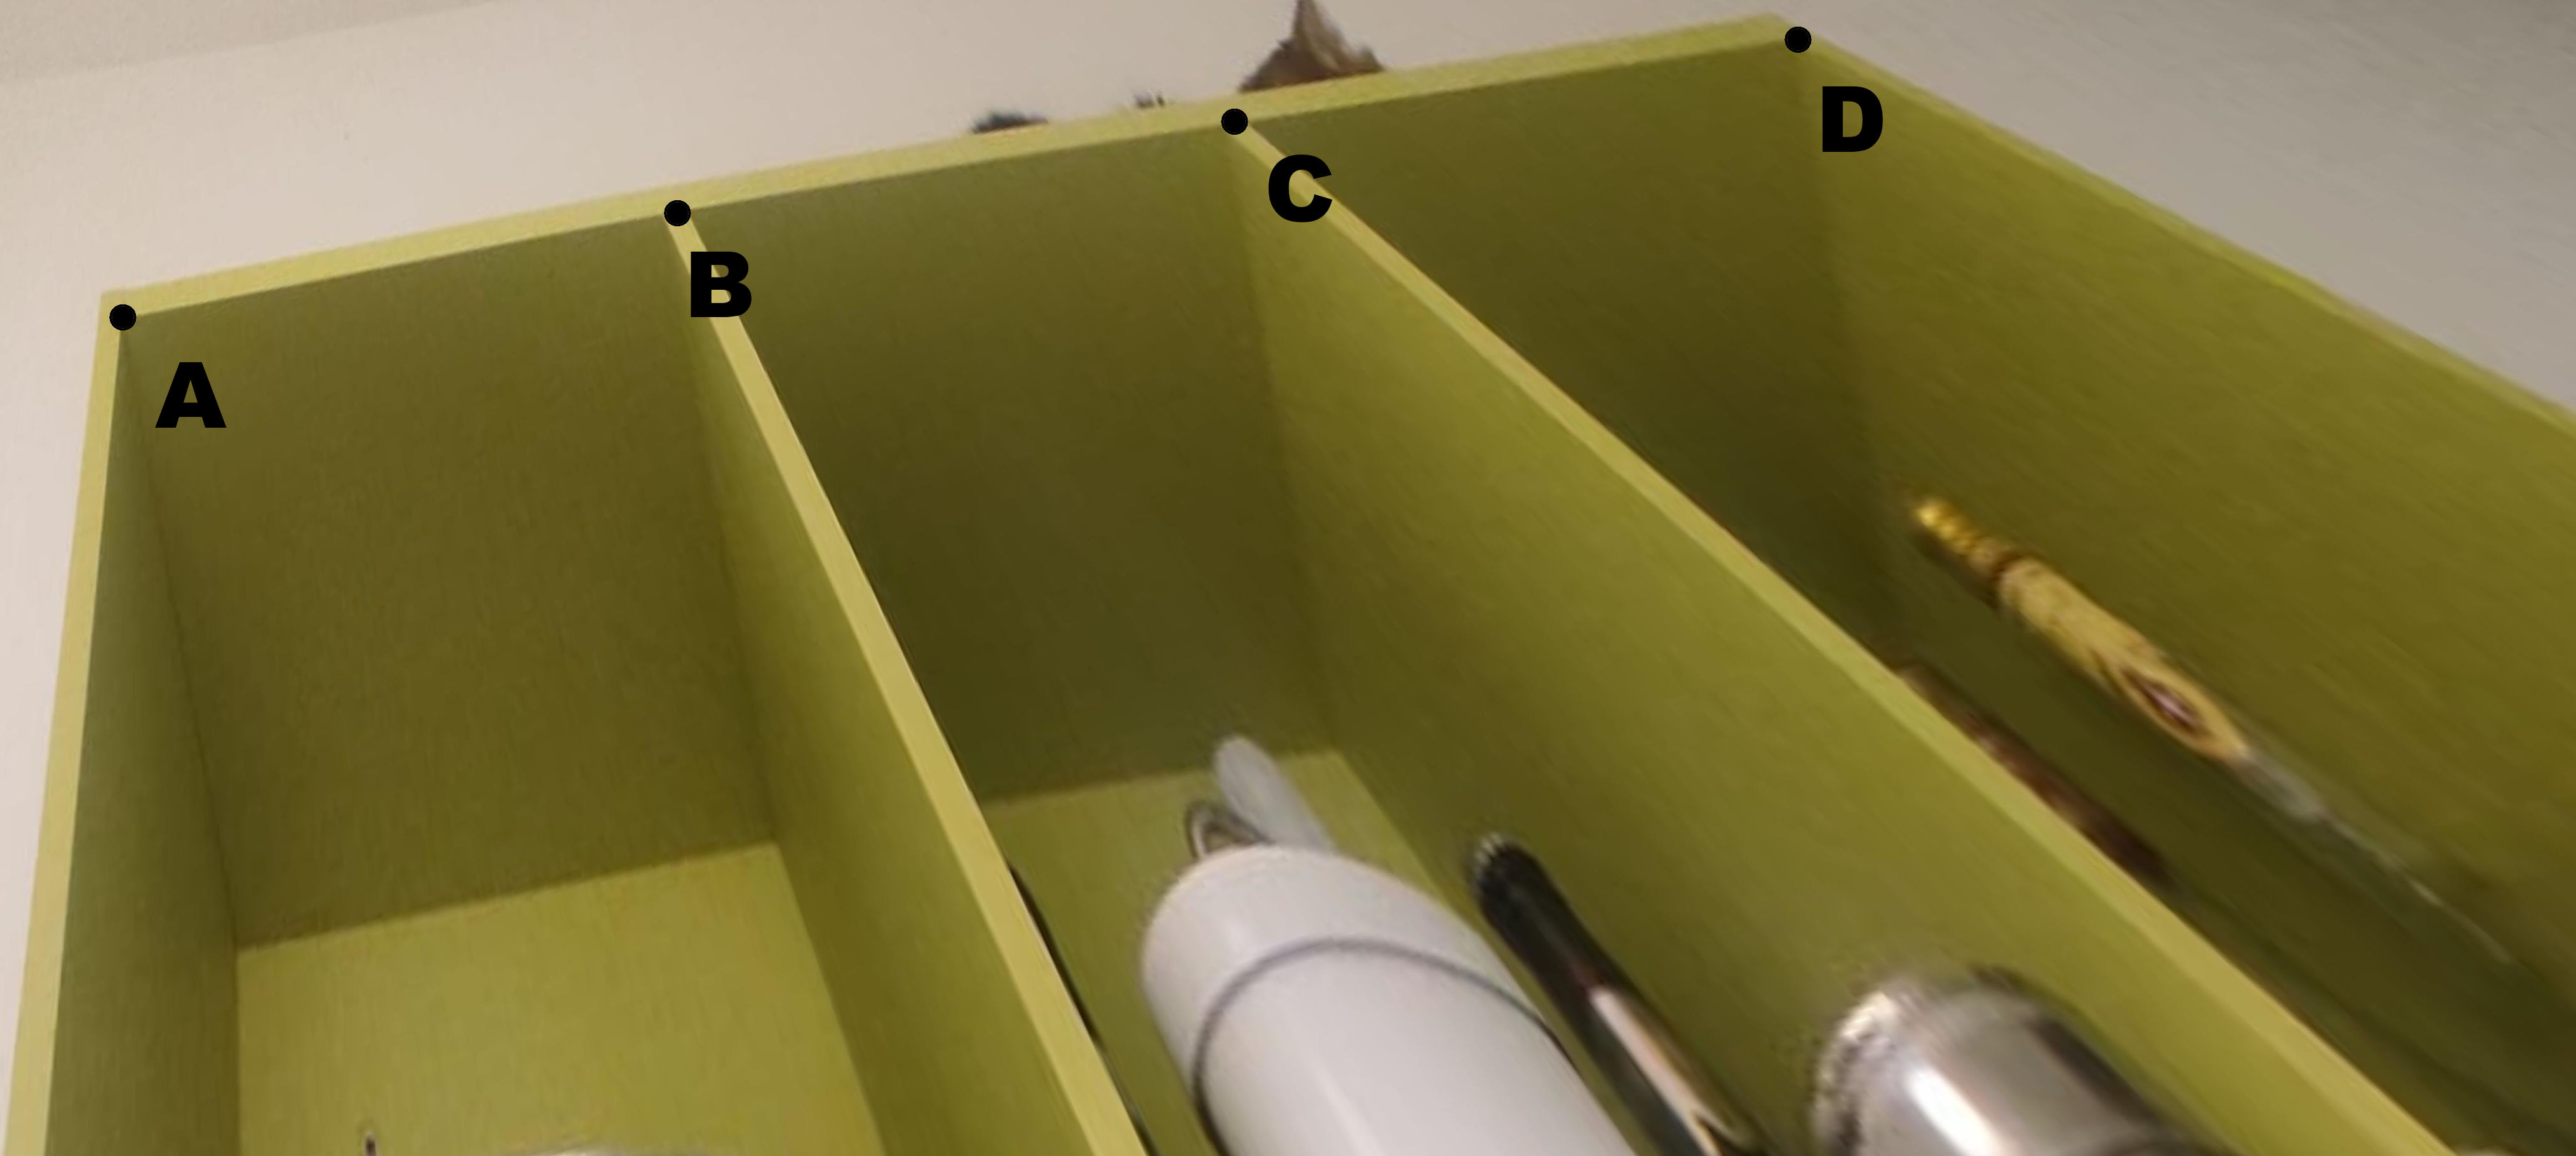
\includegraphics[width=0.7\linewidth]{img/cr.png}
    \caption{Selected points to compute $CR$}
    \label{fig:selectedPoints}
\end{figure}

In real world, based on our hypothesis we know:
\begin{itemize}
    \item $A = 0 \, m$
    \item $B = \frac{1}{3} \, n$
    \item $C = \frac{2}{3}\, m$
    \item $D = 1 \, m$
\end{itemize}

Remembering the cross ratio of a 4-tuple of collinear points formula:
$$ CR_{Y,Z,X_1,X_2} = \frac{c-a}{c-b} / \frac{d-a}{d-b}$$
\begin{figure}[H]
    \centering
    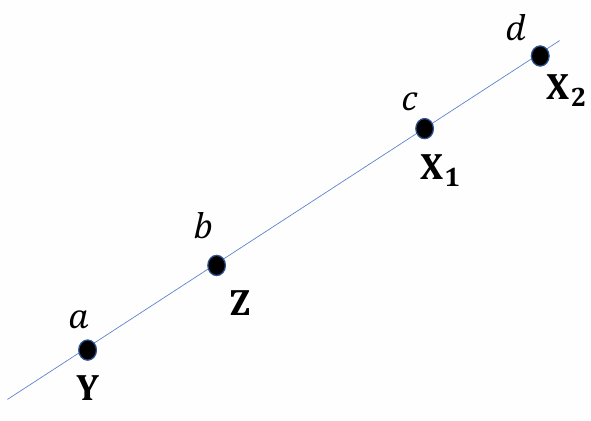
\includegraphics[width=0.5\linewidth]{img/crTheory.png}
    \caption{Cross ratio formula}
    \label{fig:crTheory}
\end{figure}

The real-world aspect ratio is computed as:

$$CR_{real} = \frac{\frac{2}{3} - 0}{\frac{2}{3} - \frac{1}{3}} / \frac{1 - 0}{1 - \frac{1}{3}} = \frac{4}{3}$$

By executing the code available in \verb|G2\cr.m|, which involves manually selecting and obtaining the pixel coordinates of the points shown in Figure \ref{fig:selectedPoints}, the image aspect ratio was determined to be:

$$CR_{image} = 1.3484 \approx \frac{4}{3}$$

Since the aspect ratio ($CR$) is preserved from the real world to the image and the computed ratios are approximately equal, we can conclude that the parallelepiped is divided into three blocks of equal length.

\paragraph{Estimation of $m$}
From the following image, which is a zoom of the metric rectified image, we can see:
\begin{itemize}
    \item lines $l_x$ and $l_y$ are parallel, as direct consequence of metric rectification, since parallel lines in the real world remain parallel in the metric rectified image 
    \item lines $m_1$ and $m_2$ are parallel, for the same reason above
    \item lines $m_1$ and $l_x$ are orthogonal, as direct consequence of the metric rectification computed
    \item lines $m_1$ and $l_y$ are orthogonal, since $m_1$ is orthogonal to $l_x$ and $l_x$ is parallel to $l_y$ 
\end{itemize}
\label{square}
So, we can clearly see that all the internal angles are right angles and we can hypothesize that the figure is a square. To confirm our hypothesis, we just measure the angle between between the intersection of the two diagonals and check if is a square one, again using the formula \ref{eq:1}.

\begin{figure}[H]
    \centering
    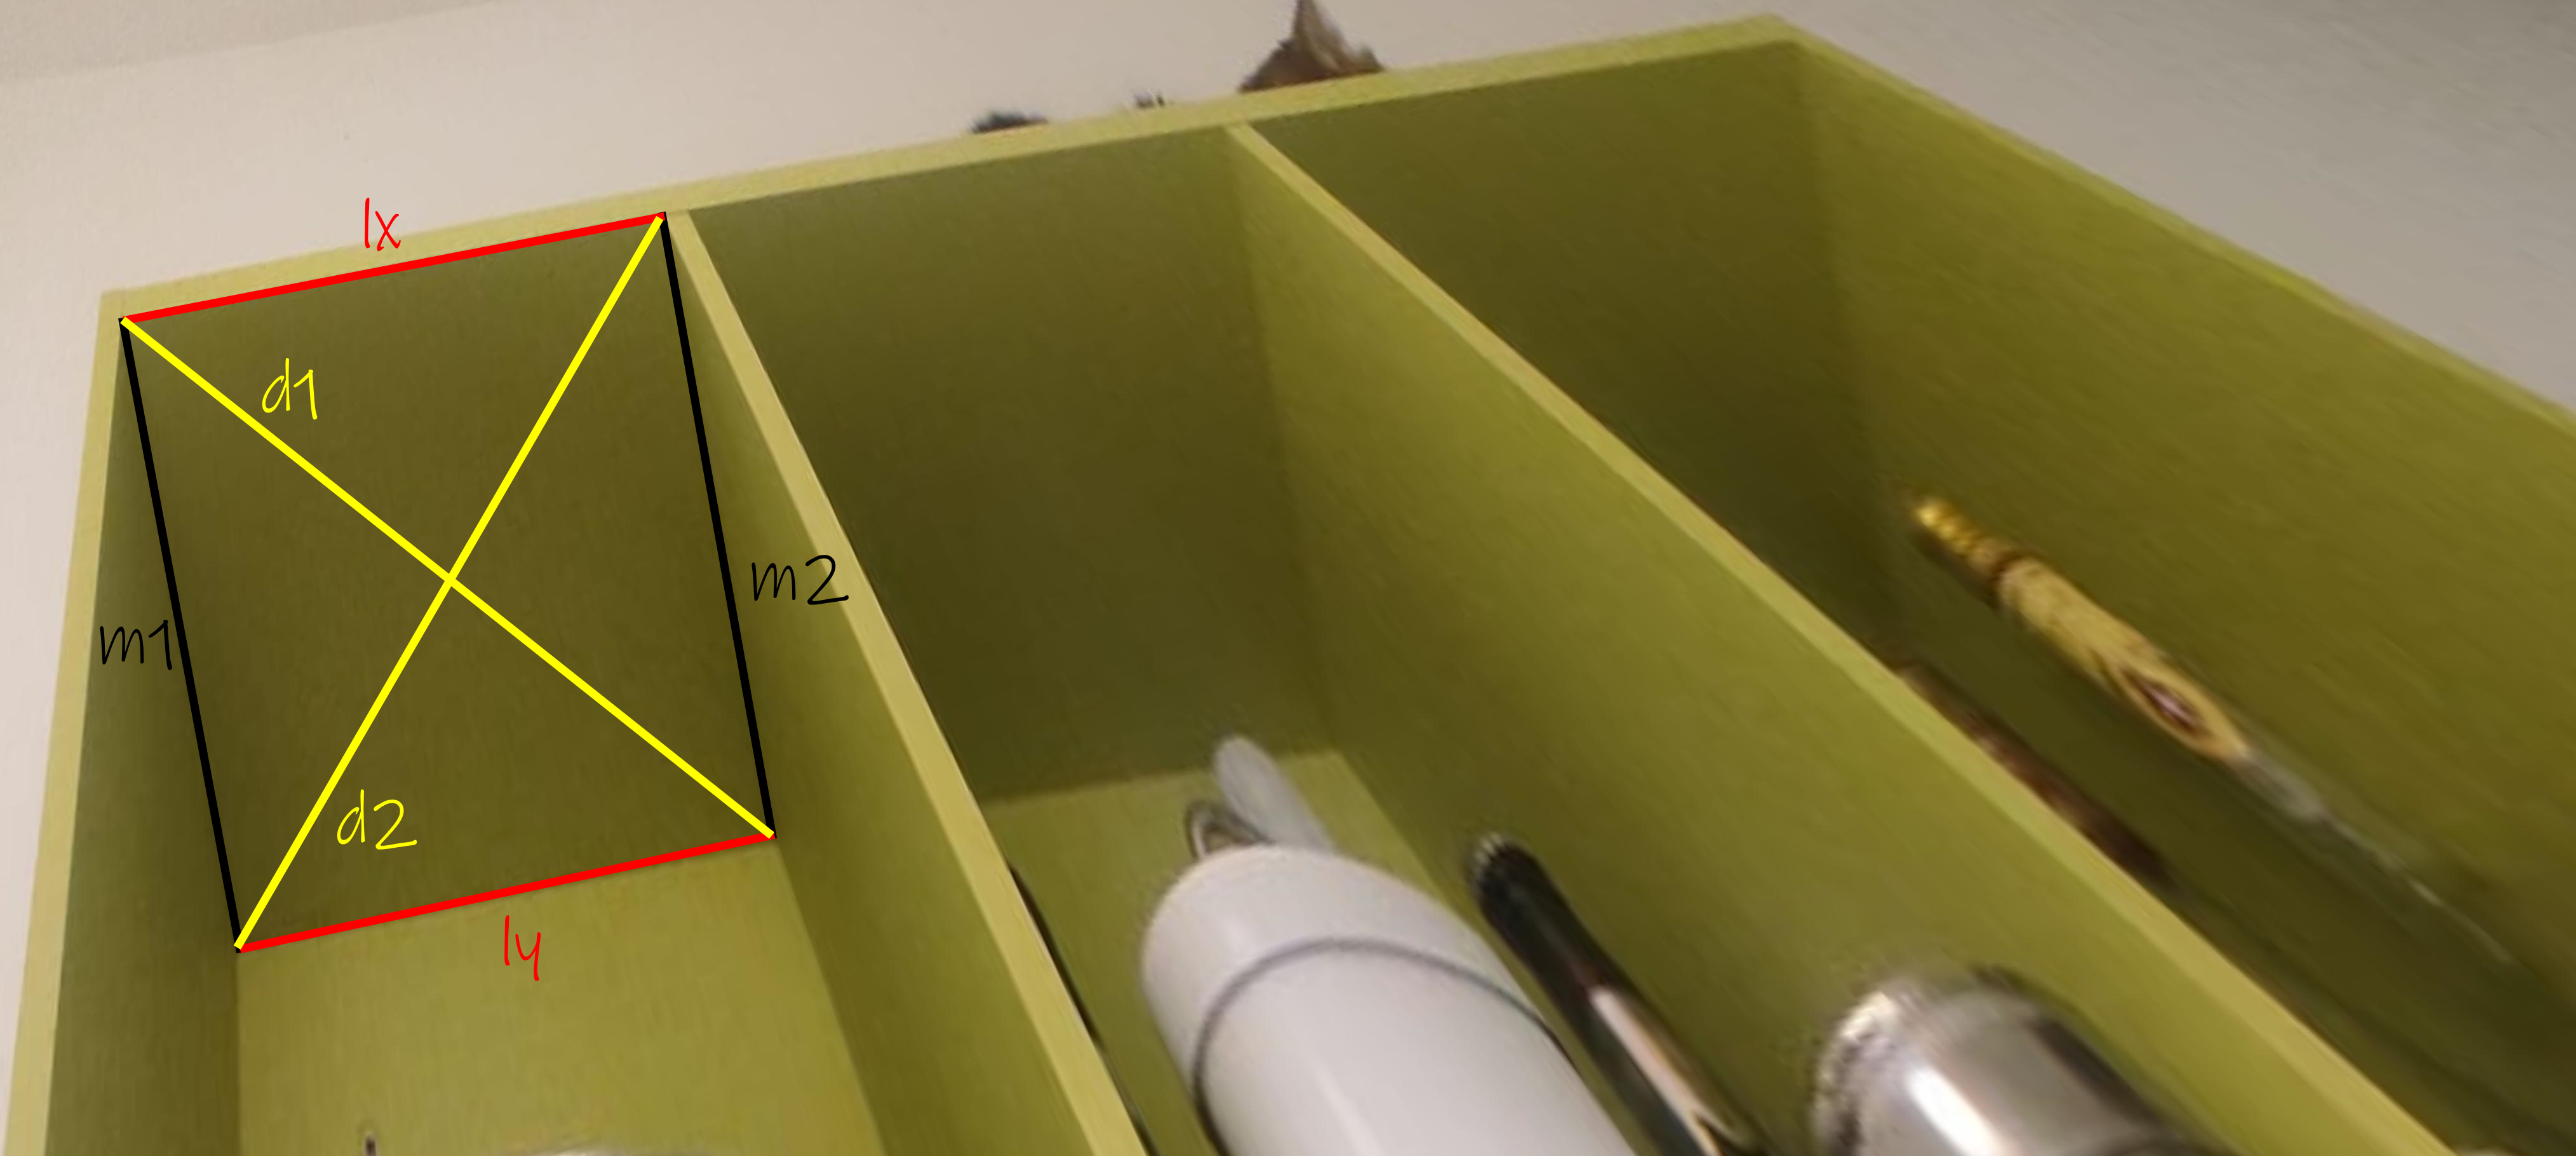
\includegraphics[width=0.5\linewidth]{img/square.png}
    \caption{Square}
    \label{fig:square}
\end{figure}

The angle computed is $\approx 98^{\circ}$, similar to a right one. We can conclude that the figure is a square and finally to conclude that the depth $m$ of the parallelepiped is equal to the length of a single block, about $\frac{1}{3}$ meter, which is a similar value to the one computed previously.

The values are not precisely the same, but they are very similar and we can conclude the depth of the parallelepiped is $\frac{1}{3}$ of the length of it.
\section{G3: Camera calibration}
In order to calibrate the camera it's necessary to select at least four constraints, since the zero skew camera was already a constraint itself, to get the \textbf{image of the absolute conic} (IAC). The IAC is strongly related to the calibration camera matrix K through the relation $w = (KK^T)^{-1}$:
\begin{equation}
    w = 
    \begin{bmatrix}
        \alpha^2 & 0 & -u_0\alpha^2 \\
        0 & 1 & -v_0 \\
        -u_0\alpha^2 & -v_0 & f_y^2 + \alpha^2u_0^2+v_0^2
    \end{bmatrix}
\end{equation}

\subsection[Vanishing point of \textit{h} lines]{Vanishing point of $h_k$ lines}
Applying the considerations in section \ref{sec:vanPoint_l} and selecting the $h_k$ lines from the original image, we obtain the following vanishing point:
\begin{equation} \label{eq: vanPoint_h}
    V_h = 
    \begin{bmatrix}
        0.6598 \times 10^{3} \\
        -1.4098 \times 10^{3} \\
        0.0010 \times 10^{3}
    \end{bmatrix}
\end{equation}

\subsection{System of equations}
Two constraints could be easily recovered by exploiting the metric rectify transformation matrix found previously (\ref{metricRectMatrix}), combined with the image of circular points $h_i \pm i \cdot h_2$:

\begin{equation}
    \begin{cases}
        h_1^Twh_2 = 0 \\
        h_1^Twh_1 - h_2^Twh_2 = 0    
    \end{cases}
\end{equation}

The other two constraints can be obtained from the vanishing point $v$ of direction perpendicular to the vertical plane $\pi$:
\begin{equation}
    \begin{cases}
        v^Twh_1 = 0 \\
        v^Twh_2 = 0    
    \end{cases}
\end{equation}

\subsection{Calibration matrix}
Obtaining the calibration matrix $K$ through Cholesky Decomposition of $w=(KK^T)^{-1}$ as:
\begin{equation} \label{eq:calibrationMatrix}
    \begin{bmatrix}
        f_x & 0 & u_0 \\
        0 & f_y & 0 \\
        0 & 0 & 1
    \end{bmatrix}
    =
    \begin{bmatrix}
        1.4896 \times 10^{3} & 0 & 0.0015 \times 10^{3} \\
        0 & 2.1845 \times 10^{3} & -0.0002 \times 10^{3} \\
        0 & 0 & 1
    \end{bmatrix}
\end{equation}
Where $f_x, \, f_y, \, u_0,\, v_0$ are the intrinsic parameters of the camera.
\section{G4: Estimation of the height of the parallelepiped}
To find the estimate value of the height of the parallelepiped, we could use a similar approach to what we have done to find the estimation of the value of the depth of the parallelepiped, explained in section (\ref{estimationDepth}).

In order to follow that approach, we have to rectify the original image in order to have a frontal view of the scene.

\subsection{Reconstruction of a frontal view}
Through the knowledge of the calibration matrix $K$, section (\ref{eq:calibrationMatrix}), we are able to compute the image of the absolute conic:
$$w=(KK^T)^{-1}$$

Then it was enough to compute again the image of the line at infinity, with respect to the vertical plane $\pi$ we were going to rectify. and intersect with the Image of the Absolute Conic.
The result led us to the Image of the two Circular Points as direct result of the equations and finally, through SVD decomposition, we bring them to their canonical position in purpose of obtaining the desired vertical plane rectified.

\begin{figure}[H]
    \centering
    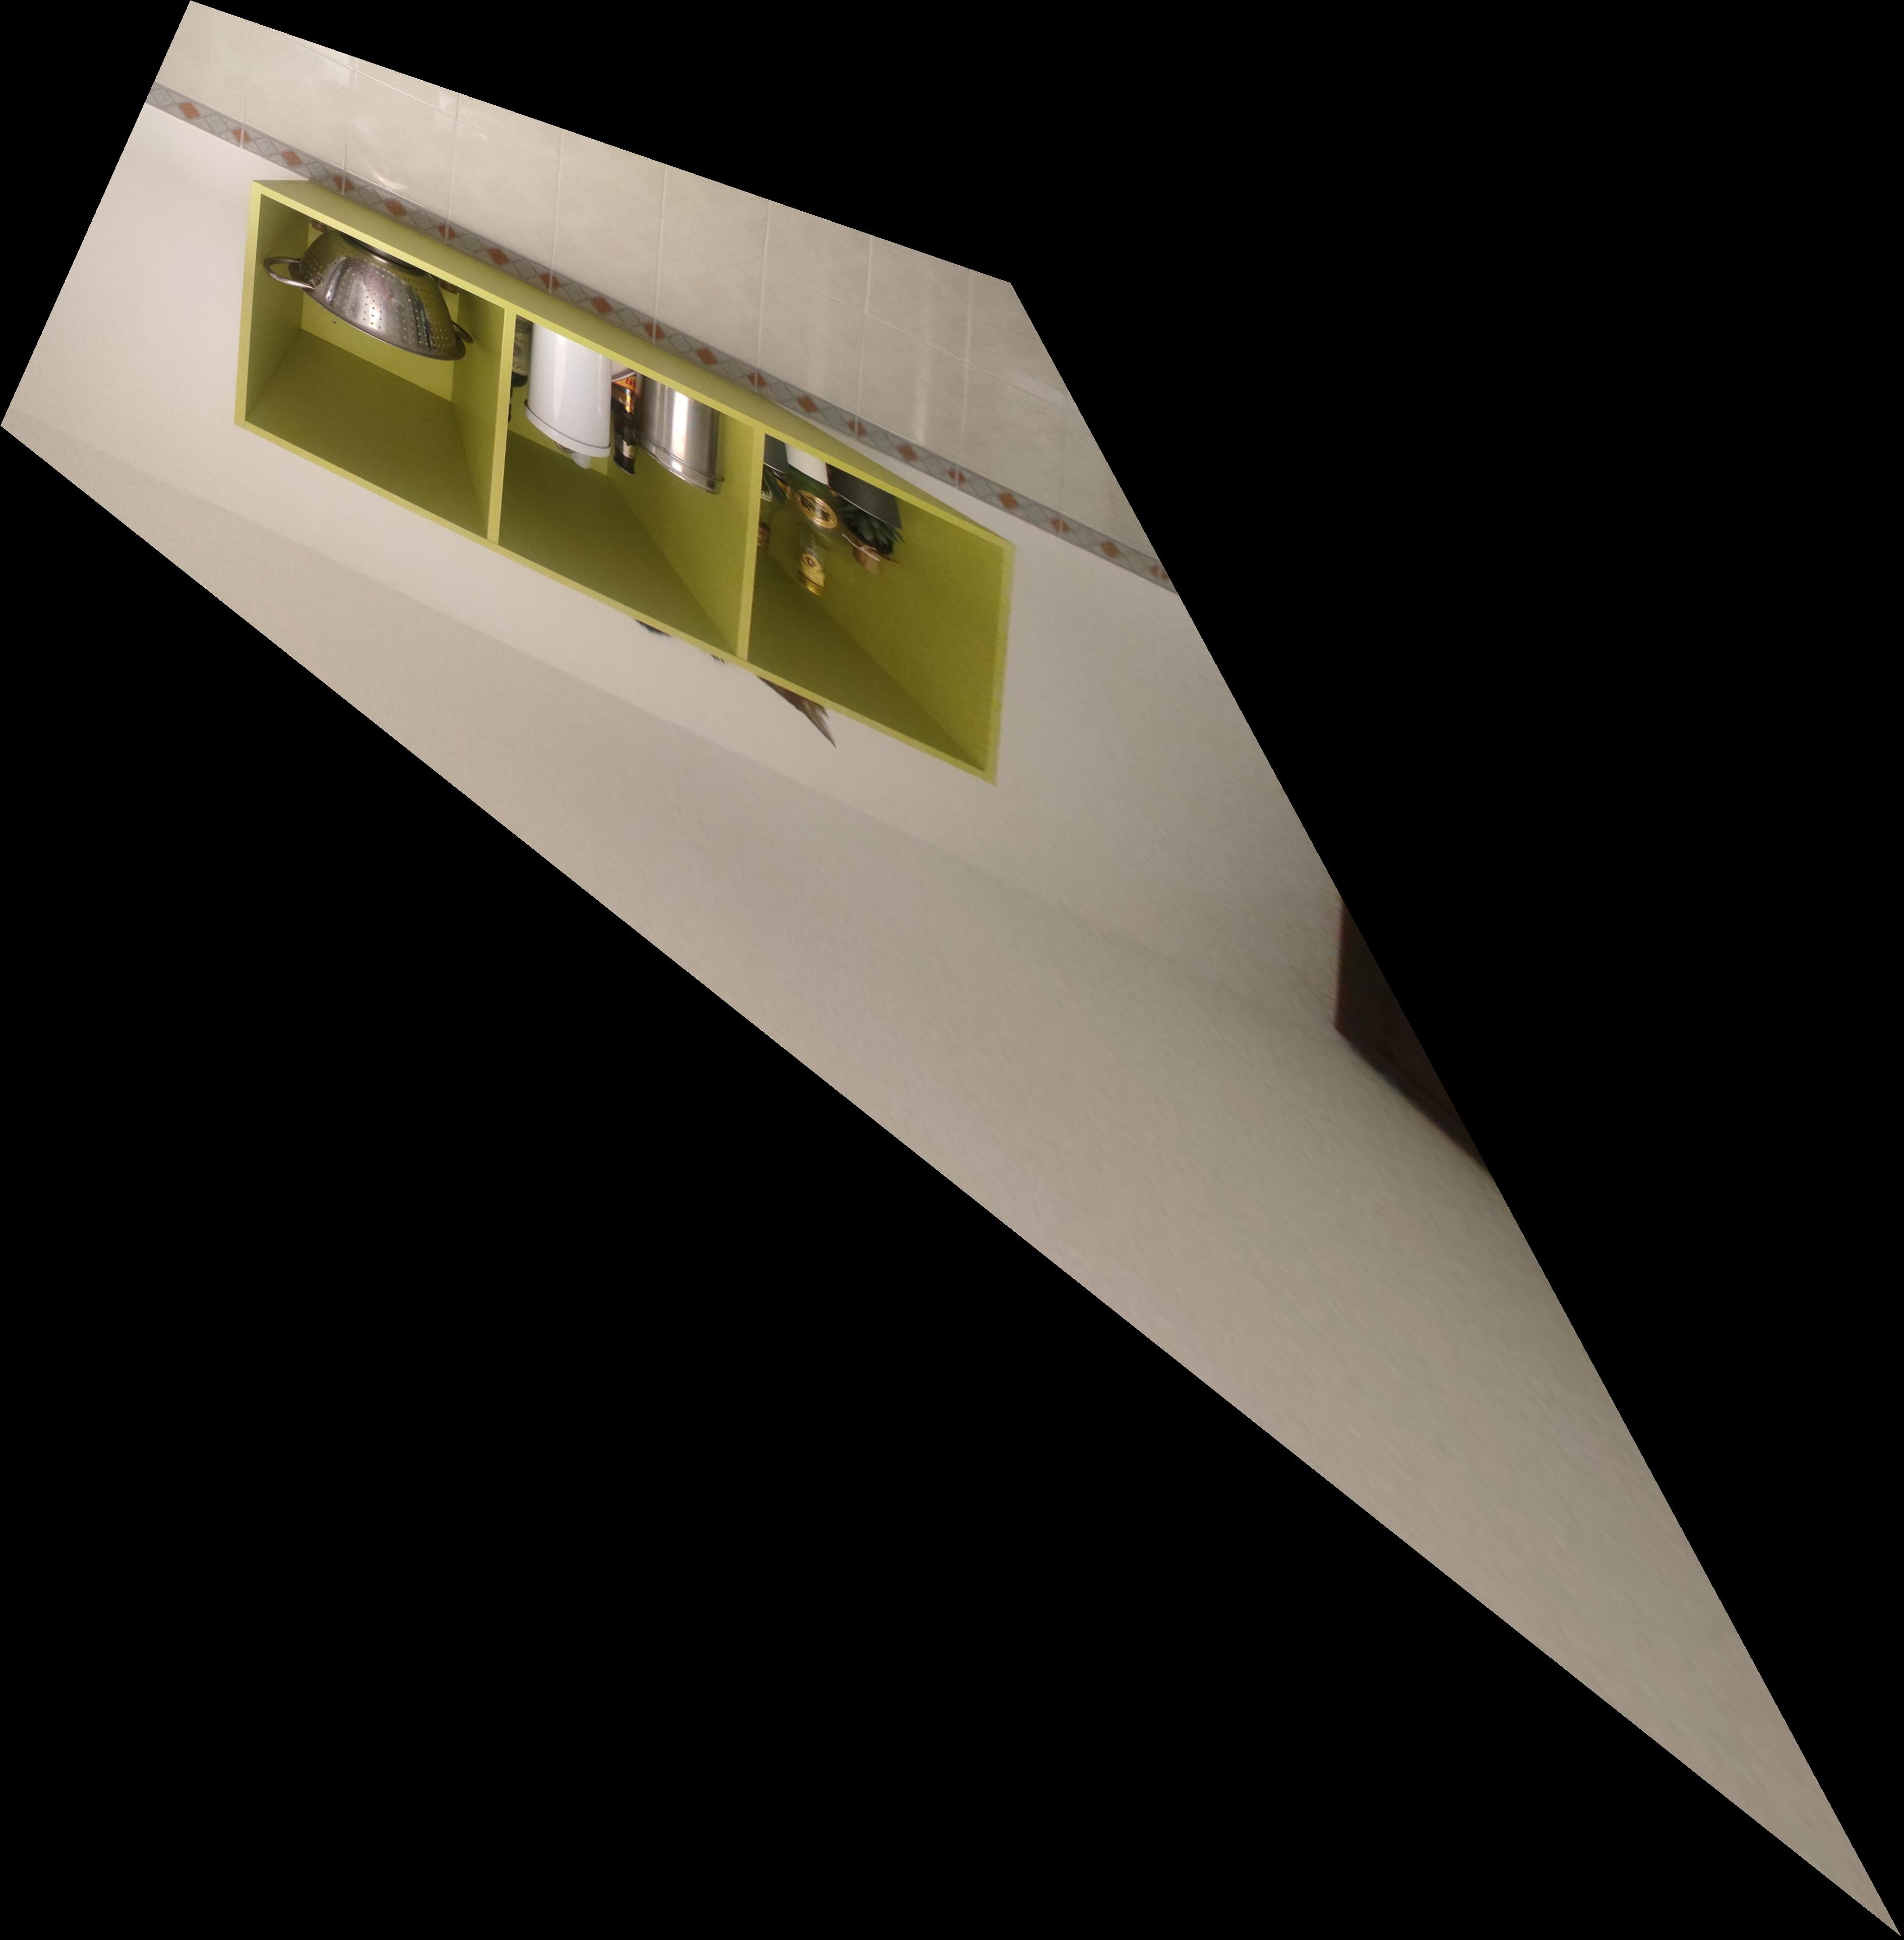
\includegraphics[width=0.95\linewidth]{img/G3/verticalReconstructionK.jpg}
    \caption{Reconstructed vertical plane using $K$}
    \label{fig:verticalRectK}
\end{figure}

\subsection{Estimation of height}
Following the same approach used to determine the depth of the parallelepiped, we can measure $\cos\gamma$ using formula \ref{eq:1} shown in the figure. Knowing that $l_x$ and $h_y$ should form a right angle and given $l = 1 \, \mathrm{m}$, we can compute the numerical value of the height as:

\[
h = l \sqrt{1 - \cos^2\gamma}
\]

Before proceeding with the numerical computation of $h$, it is crucial to verify, in the rectified image, whether the angle between $l$ and $h$ is indeed a right angle. Using a simple program to calculate the angle between two lines, we can verify that $l$ and $h$ are not perfectly perpendicular. This discrepancy arises due to numerical instability and inaccuracies in the matrix $K$.

\subsubsection{2D Reconstruction of the Vertical Plane}
In order to obtain a more precise reconstruction of the vertical plane, we follow the typical approach, using metric-stratified method, selecting $l$ and $m$ lines from the provided image in order to build the affine rectified image and finally selecting, from the obtained result, two pairs of orthogonal and independent lines as shown in the following pictures:

\begin{figure}[H]
     \centering
     \begin{subfigure}[b]{0.45\textwidth}
         \centering
         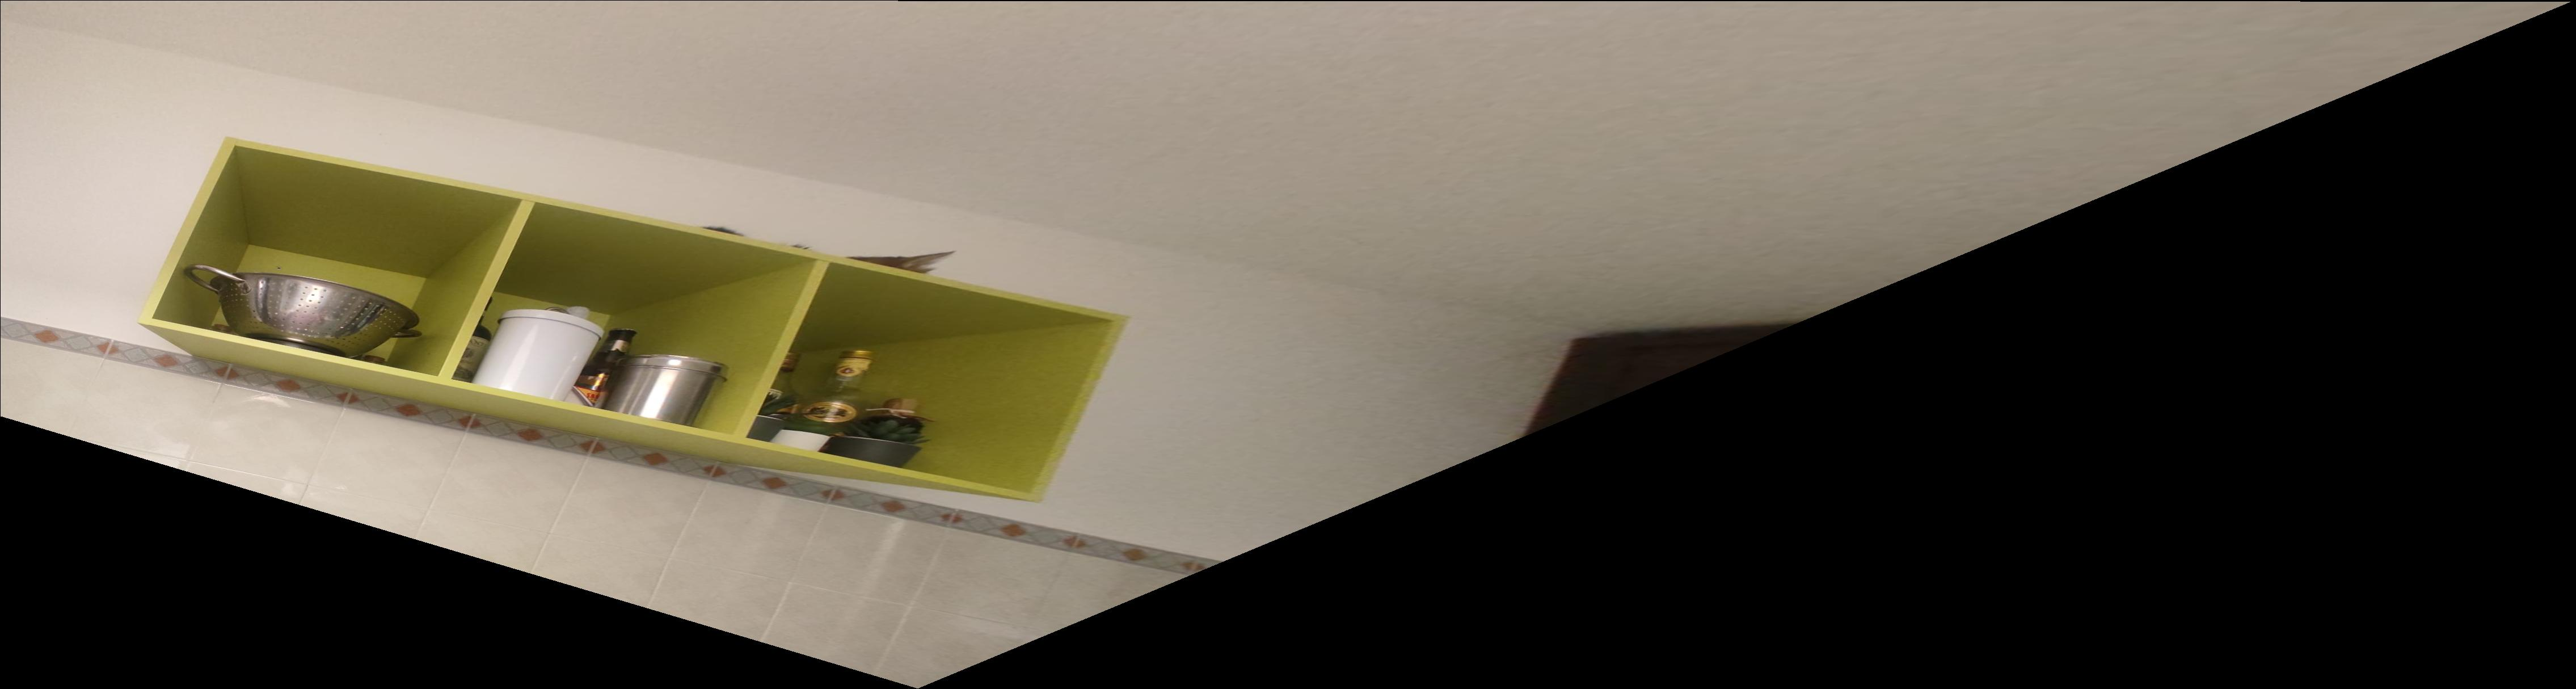
\includegraphics[width=\textwidth]{img/G3/affineVertRectification.jpg}
         \caption{Affine Rectification}
     \end{subfigure}
     \hfill
     \begin{subfigure}[b]{0.45\textwidth}
         \centering
         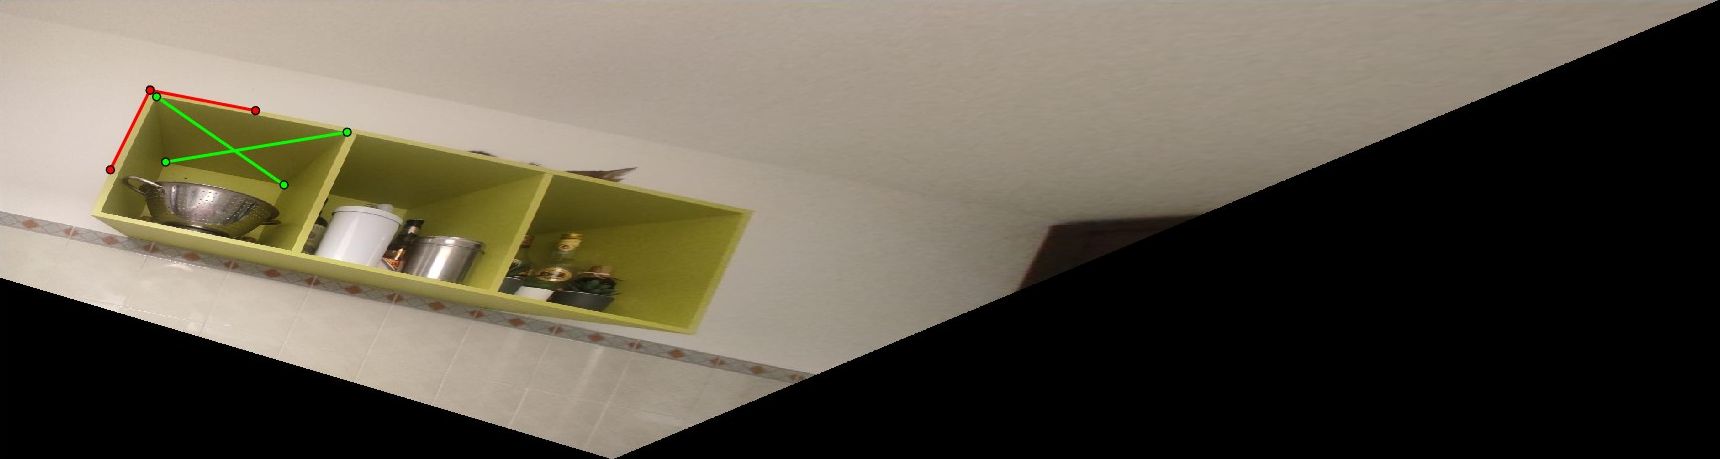
\includegraphics[width=\textwidth]{img/G3/affineWithLines.png}
         \caption{Pairs of orthogonal and independent lines}
         \label{pairOrthogonalLines}
     \end{subfigure}
\end{figure}

Note that the lines in Figure \ref{pairOrthogonalLines} can be selected because, as shown in (\ref{square}), the green lines are the diagonals of a square and are therefore orthogonal.

The rectified image obtained is:
\begin{figure}[H]
    \centering
    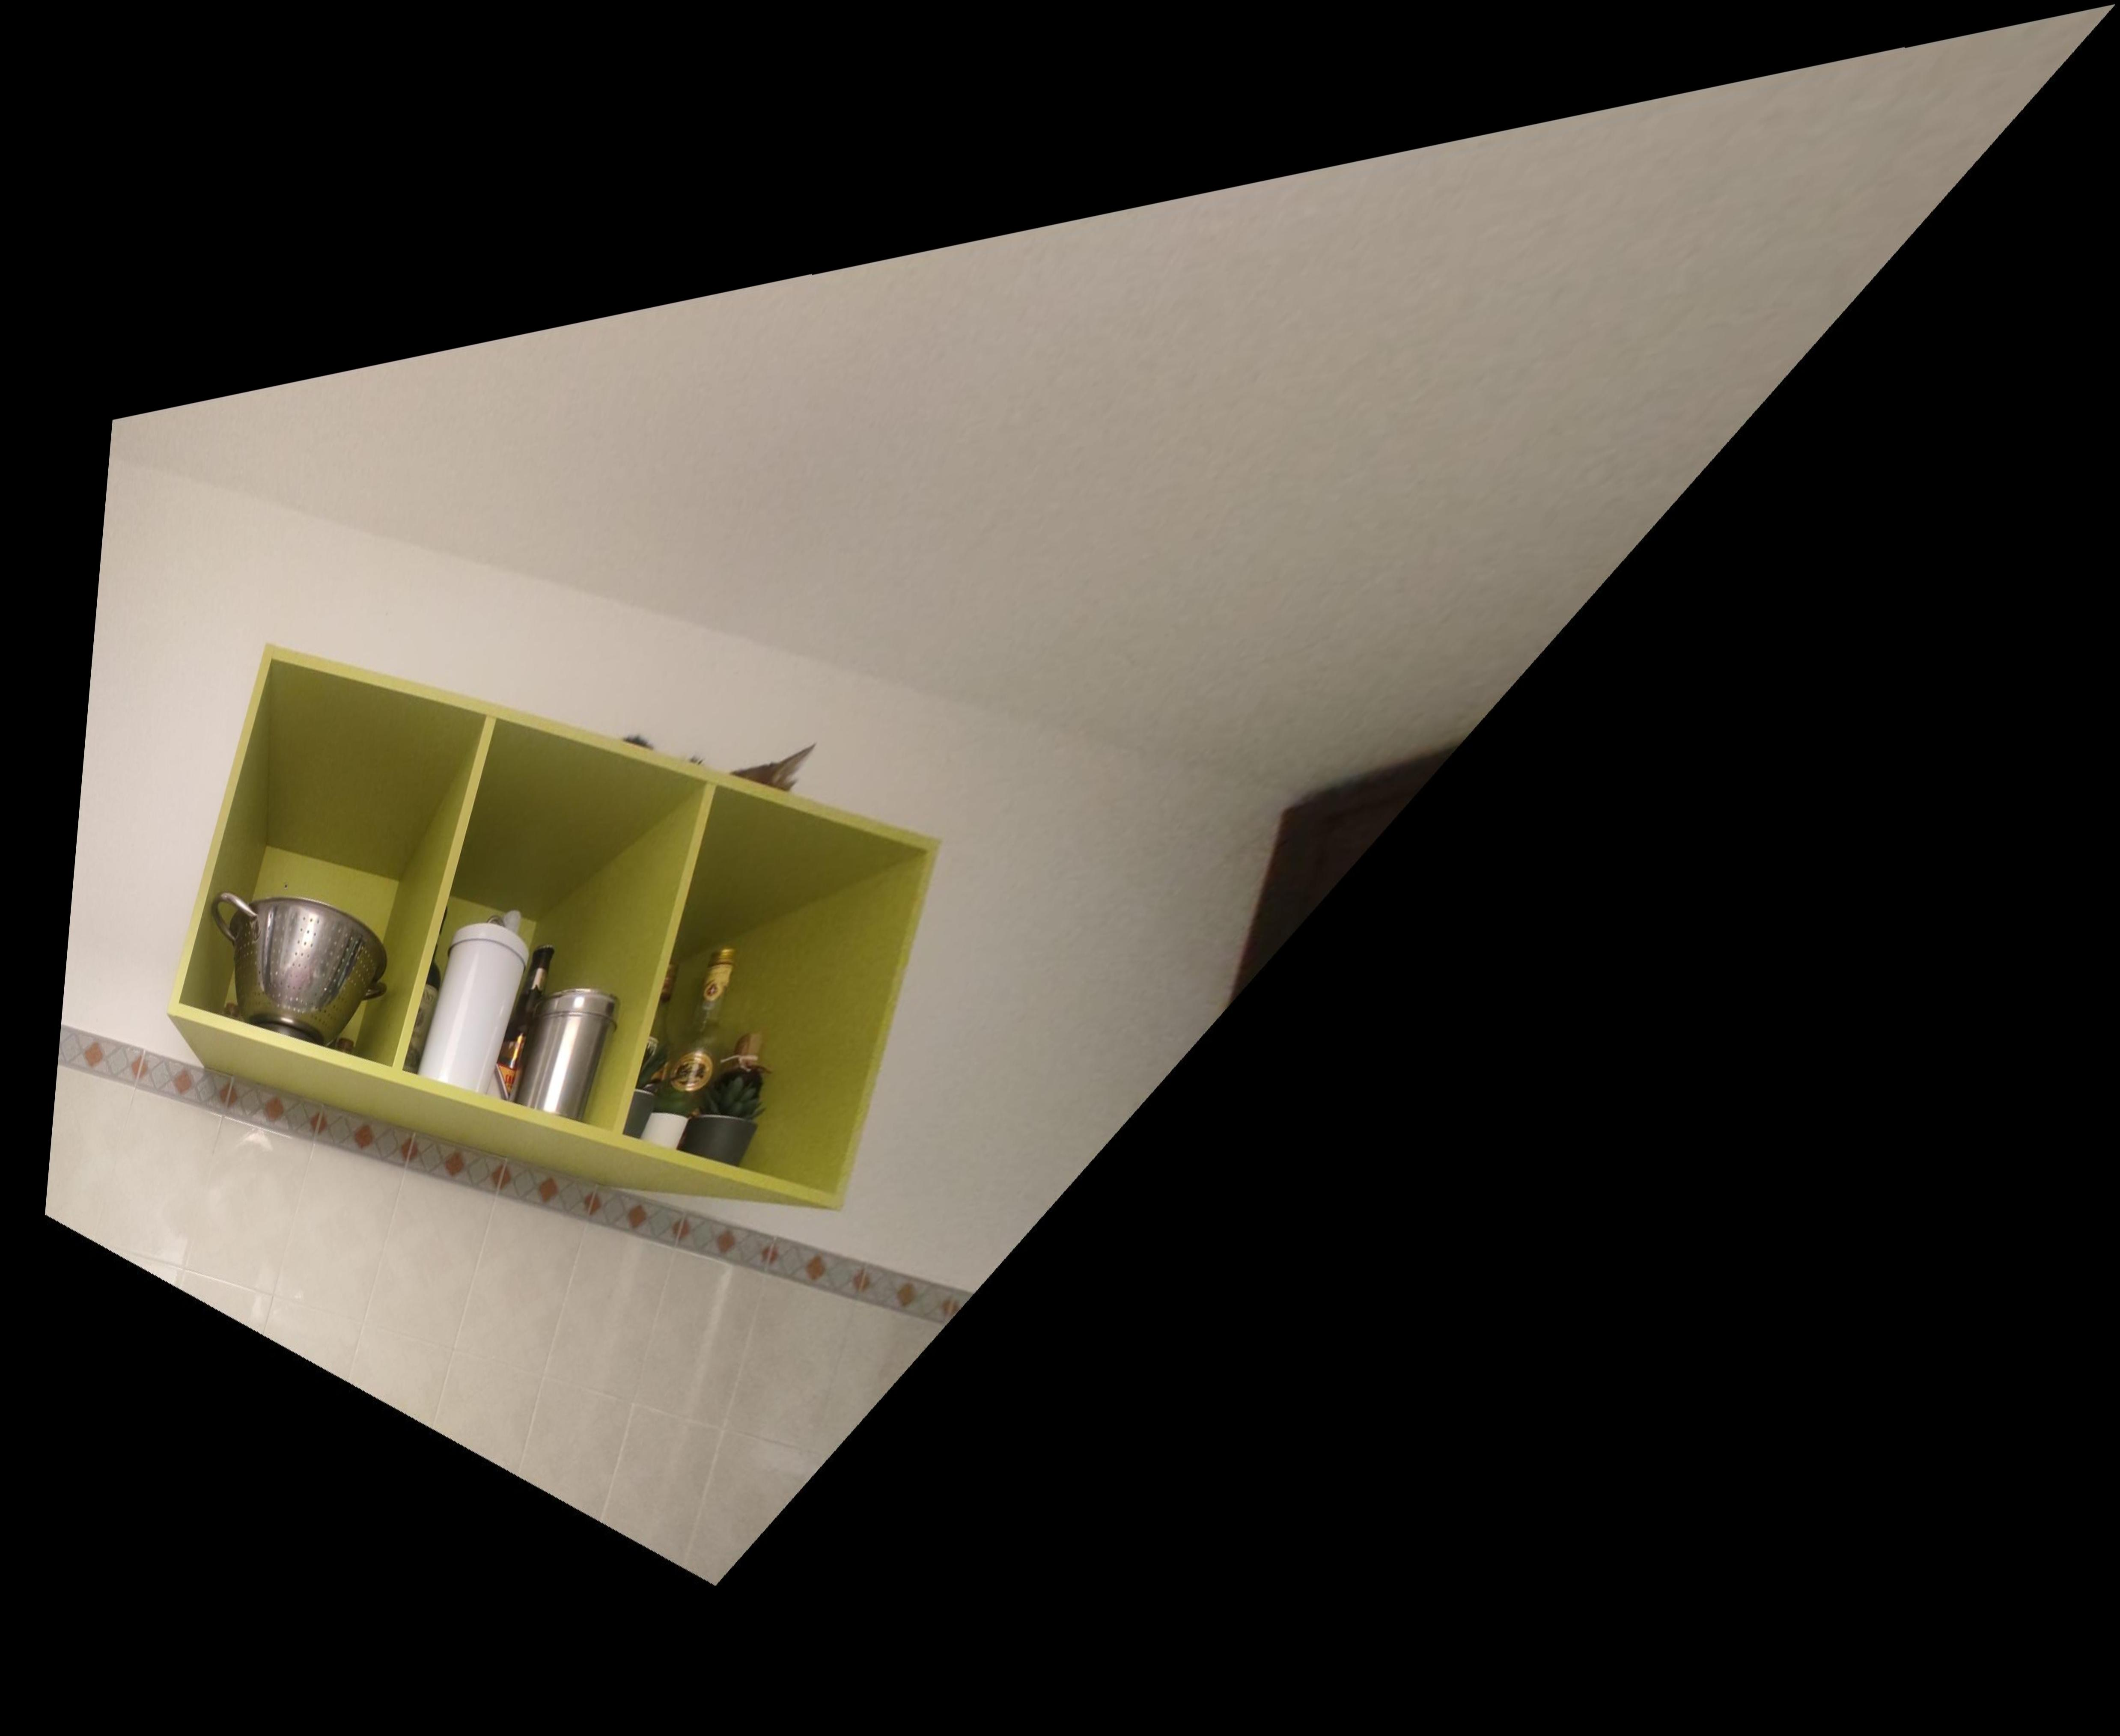
\includegraphics[width=0.75\linewidth]{img/G3/verticalRectificationMetric.jpg}
    \caption{Vertical Rectification}
    \label{fig:verticalRectMetric}
\end{figure}

\subsubsection{Compute $h$}
The obtained result is slightly improved compared to the previous one, as the computed angle between the $l$ and $h$ lines is very close to $90^\circ$. This allows us to calculate a more accurate numerical value for the height of the parallelepiped. The same method used to determine its depth, detailed in Section \ref{estimationDepth}, is applied here. Using the Pythagorean theorem for a right triangle, the $l$ and $h$ lines are defined as the two catheti, we found:

$$h \approx 0.5 \, m$$
\section[G5: \textit{X-Y} coordinates of a dozen points of \textit{S}]{G5: \textit{X-Y} coordinates of a dozen points of $S$}
This section focuses on the computation and visualization of $X-Y$ coordinates for selected points on the curve SS, leveraging a metric-rectified image from previous stages. The objective is to map curve points from their original image space to a rectified coordinate space, ensuring metric accuracy, and to visualize the adjusted curve points on the rectified image.

\begin{itemize}
    \item \textbf{Rectified Image}: The metric-rectified image (\ref{fig:metricRectificationUsingOneCircle}) obtained in previous steps was loaded as the base for the analysis.
    \item \textbf{Curve SS Points}: Data points defining the curve $S$ were read from input file. These points are assumed to be in the original image's pixel space.
\end{itemize}

A set of known reference points in the original image and their corresponding points in the rectified image were defined. These pairs were used to compute the transformation matrix.

A projective transformation (\texttt{fitgeotrans}) was computed using the reference points from the original and rectified images. This transformation was applied to map the curve $S$ points from the original to the rectified coordinate space. Using the computed transformation, the curve points were rectified.

The rectified image was displayed with the transformed curve $S$ points overlaid in red:

\begin{figure}[H]
    \centering
    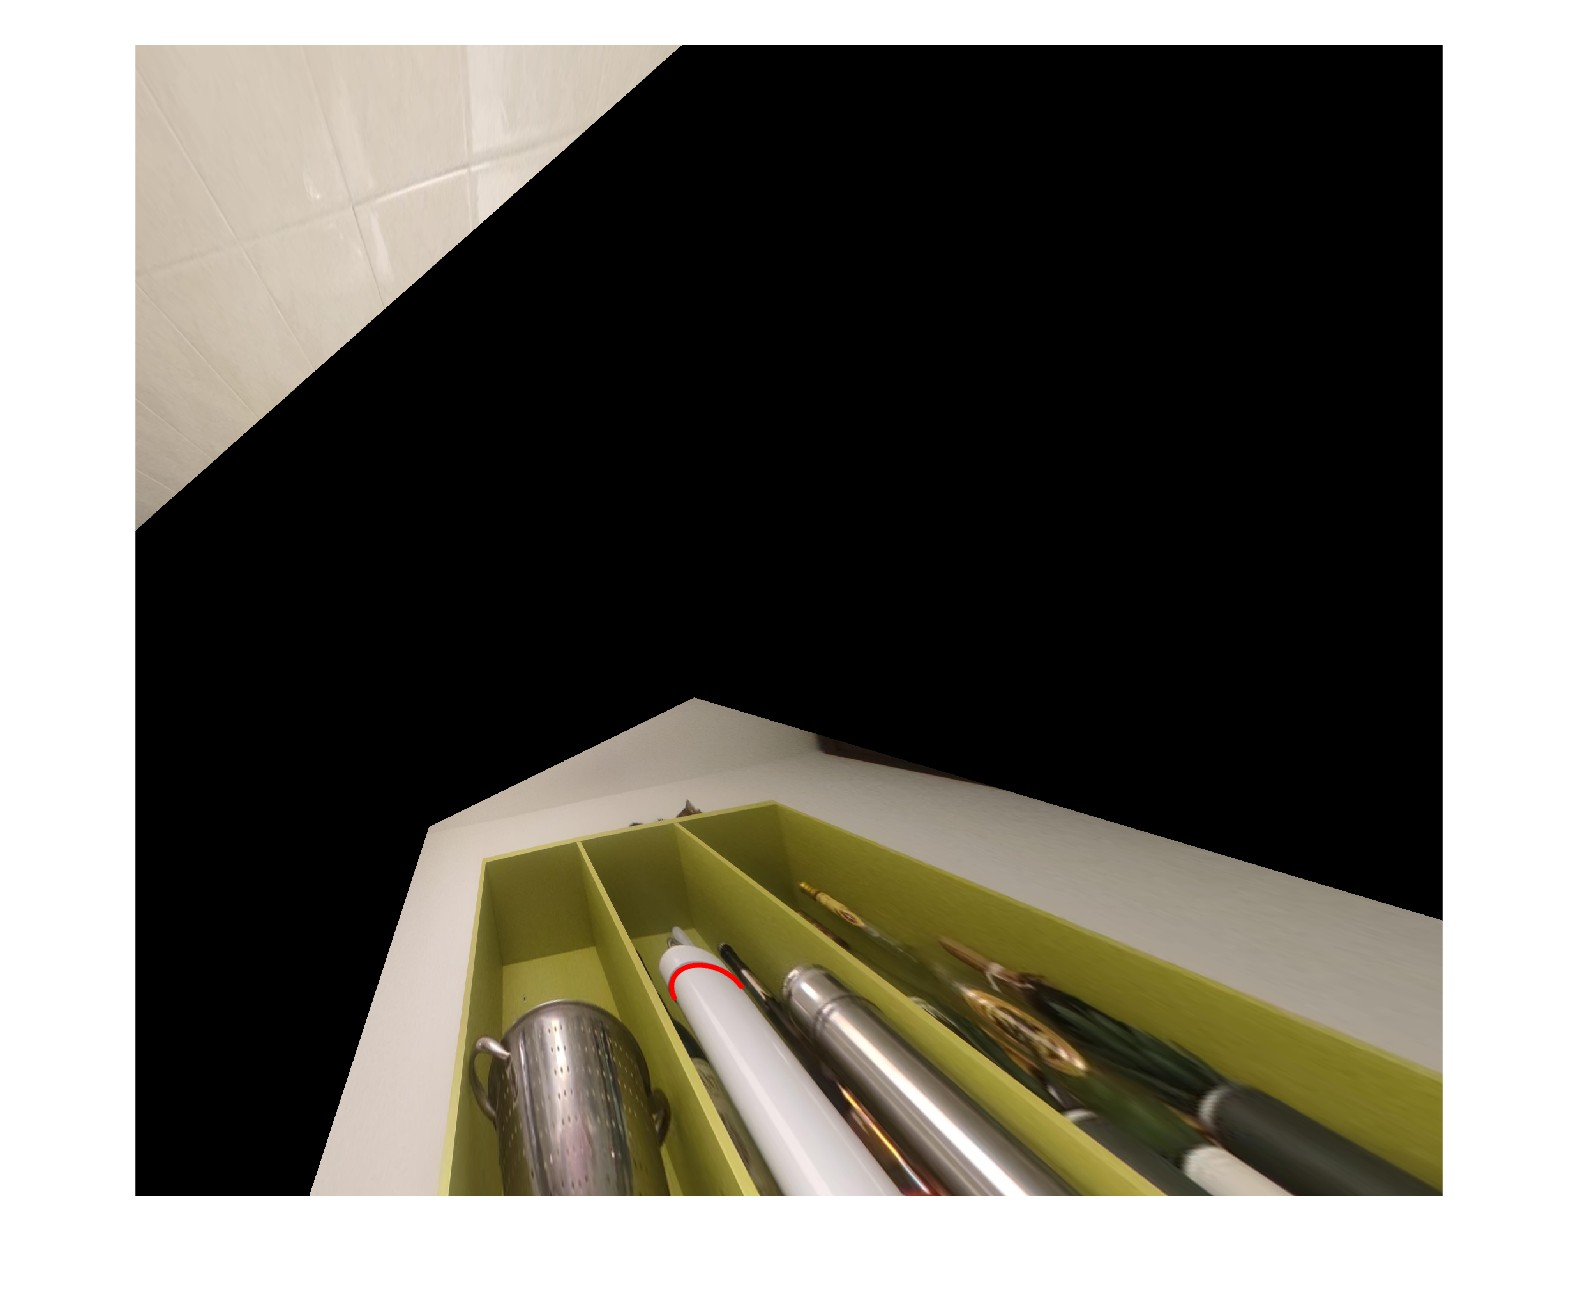
\includegraphics[width=0.7\linewidth]{img/G5/G5_horizontal_metric_rectified_with_S.jpg}
    \caption{Rectified $S$}
    \label{fig:rectifedS}
\end{figure}

To validate the rectification process and transformation accuracy, a selection of random points from the rectified curve $S$ is displayed below:

\begin{table}[h!]
\centering
\begin{tabular}{@{}c c@{}}
\toprule
\textbf{X Coordinate (in pixels)} & \textbf{Y Coordinate (in pixels)} \\ \midrule
5.4979 & 9.5996 \\
5.4950 & 9.6679 \\
6.1065 & 9.5406 \\
5.4942 & 9.6590 \\
5.6008 & 9.4646 \\
6.1350 & 9.5641 \\
5.9547 & 9.4576 \\
5.6890 & 9.4320 \\
5.5107 & 9.7314 \\
5.4937 & 9.6502 \\
6.0864 & 9.5260 \\
5.4936 & 9.6415 \\ \bottomrule
\end{tabular}
\caption{Coordinates of random points from the rectified curve \( S \), scaled by \( 10^3 \).}
\end{table}

\section{G6: Camera localization}
The goal of this chapter is to localize a calibrated camera relative to a parallelepiped using a single image and known correspondences between \verb|3D| world points and their \verb|2D| projections. The final objective is to determine the camera's extrinsic parameters: the rotation matrix and translation vector, which define the camera's pose in the world coordinate system.

From the previously requests, we know:
\begin{itemize}
    \item the length of the parallelepiped: $l = 1 \, meter$
    \item the depth of the parallelepiped: $m \approx \frac{1}{3} \, meter$
    \item the height of the parallelepiped: $h \approx \frac{1}{2} \, meter$
    \item the camera calibration matrix $K$
\end{itemize}

\paragraph{Reference System}

I decide to consider the following reference system:
\begin{itemize}
    \item X-axis runs along the edge of the length
    \item Y-axis runs along the edge of the depth
    \item Z-axis runs vertically along the edge of the height
\end{itemize}

Defining the \verb|3D| real world points and the respective one in the image, I aim to find the $3 \times 4$ projection matrix which execute the correct mapping.

This is achieved using the Direct Linear Transformation method. It emphasizes constructing the design matrix $A$, solving for $P$ using Singular Value Decomposition (SVD), and interpreting $P$ as the key to extracting the camera's extrinsic parameters.

The \textbf{camera rotation matrix} found is:
\[
    R
    =
    \begin{bmatrix}
        -0.9451 & 0.4853 & -0.0503 \\
        -0.1257 & -0.3673 & -0.9177 \\
        -0.4135 & -0.7935 & 0.3940
    \end{bmatrix}
\]

The \textbf{camera translation vector} is:
\begin{equation}
    t =
    \begin{bmatrix}
        -0.1501 \\
        -0.2444 \\
        -0.7489
    \end{bmatrix}
\end{equation}
   
To enhance the understanding of the obtained result, we visualize the camera within a \verb|3D| model:
\begin{figure}[H]
     \centering
     \begin{subfigure}[b]{0.49\textwidth}
         \centering
         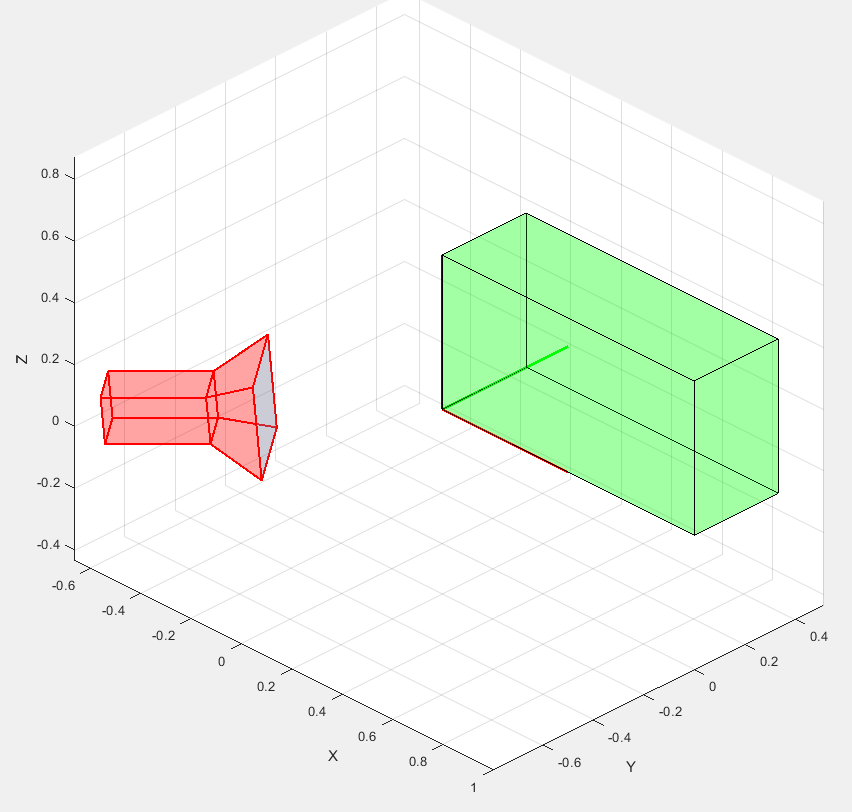
\includegraphics[width=\textwidth]{img/G6/loc1.jpg}
         \caption{Camera localization}
     \end{subfigure}
     \hfill
     \begin{subfigure}[b]{0.49\textwidth}
         \centering
         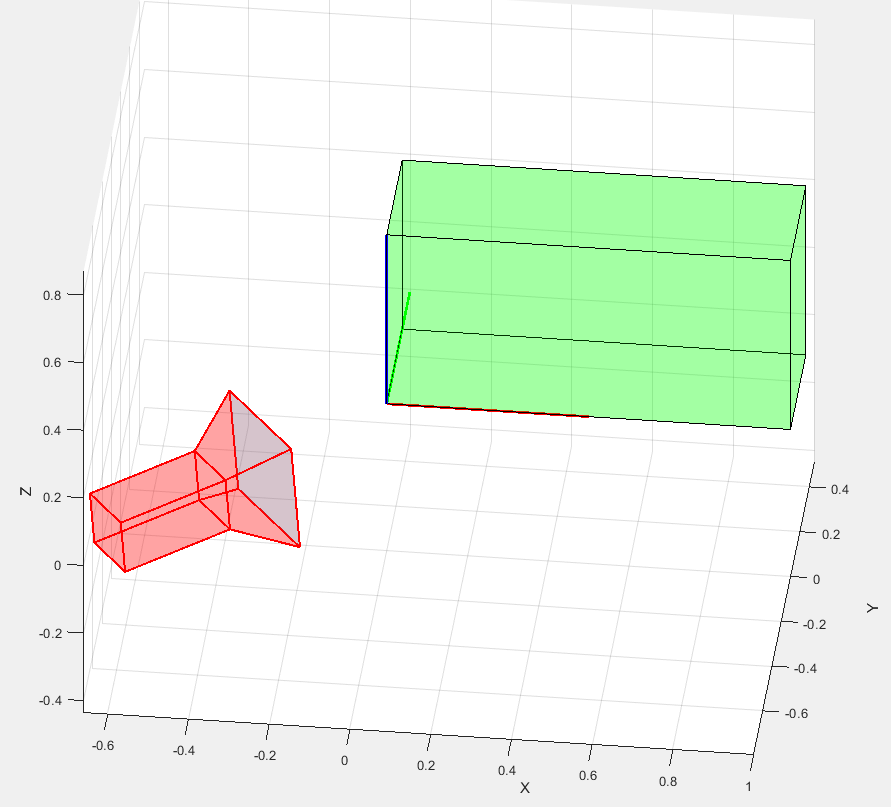
\includegraphics[width=\textwidth]{img/G6/loc2.jpg}
         \caption{Camera localization from a different view}
     \end{subfigure}
\end{figure}
\chapter{3D Model of the Parallelepiped}

As shown in the images, to enhance the understanding of the scene, I chose to colour the back wall of the parallelepiped black and render it empty. This decision was made to improve the visibility of the depth.

The recovered \verb|3D| model of the rectangular parallelepiped is displayed.

\begin{figure}[H]
     \centering
     \begin{subfigure}[b]{0.4\textwidth}
         \centering
         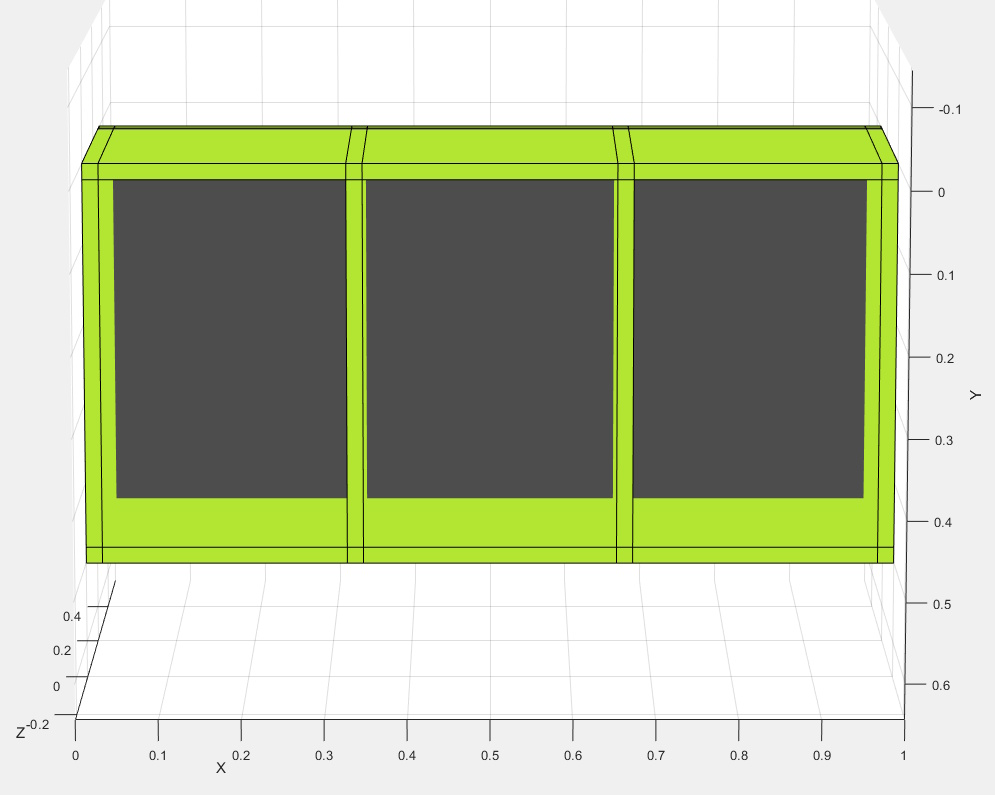
\includegraphics[width=\textwidth]{img/3d_1.jpg}
         \caption{3D model - View 1}
     \end{subfigure}
     \hfill
     \begin{subfigure}[b]{0.4\textwidth}
         \centering
         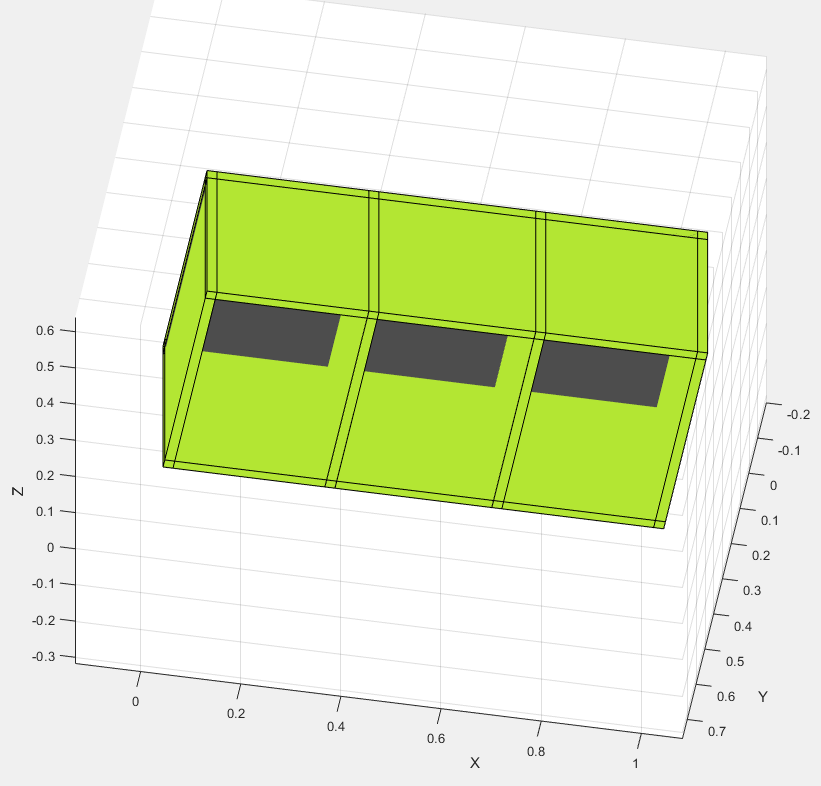
\includegraphics[width=\textwidth]{img/3d_3.jpg}
         \caption{3D model - View 2}
     \end{subfigure}
\end{figure}

\begin{figure}[H]
    \centering
    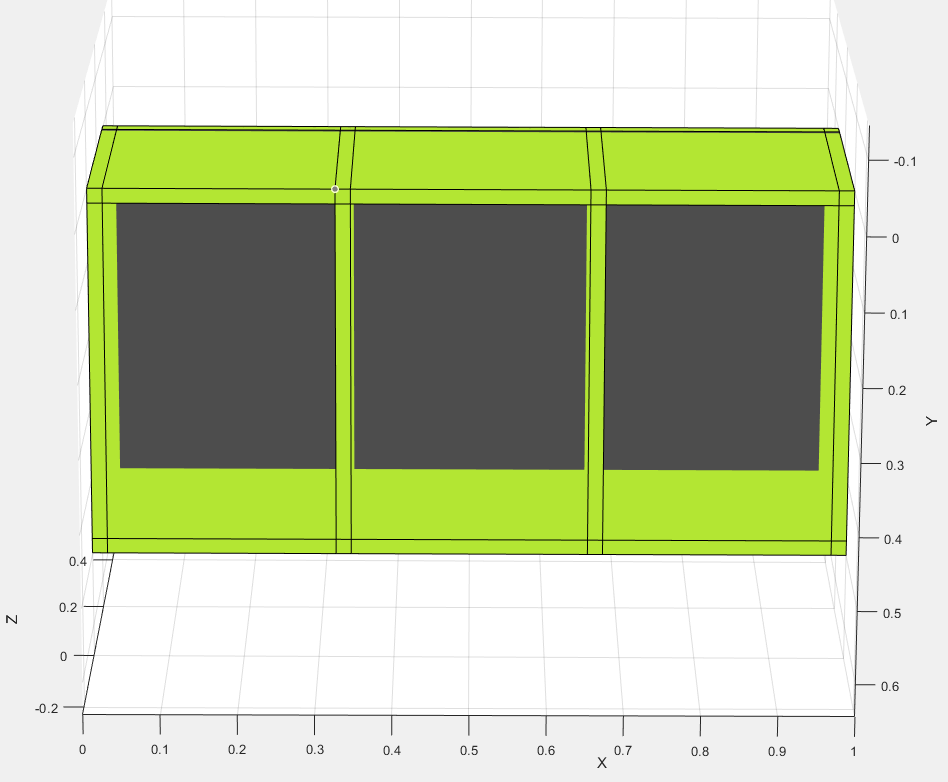
\includegraphics[width=0.5\linewidth]{img/3d_2.jpg}
    \caption{3D model - View 3}
\end{figure}

\listoffigures

\cleardoublepage

\end{document}